%%%%% Document Setup %%%%%%%%

\documentclass[12pt, twocolumn]{revtex4-1}    % Font size (12pt) and column number (one or two).

\usepackage[a4paper, left=2.5cm, right=2.5cm, top=2.5cm, bottom=2.5cm]{geometry}  % Defines paper size and margin length

\usepackage{ragged2e}

\renewcommand{\baselinestretch}{1}     % Defines the line spacing

\usepackage[caption=false]{subfig}

\usepackage{graphics,graphicx,epsfig,ulem}		% Makes sure all graphics works
\usepackage{amsmath} 						% Adds mathematical features for equations

\usepackage{etoolbox}                       % Customise date to preferred format
\makeatletter
\patchcmd{\frontmatter@RRAP@format}{(}{}{}{}
\patchcmd{\frontmatter@RRAP@format}{)}{}{}{}
\renewcommand\Dated@name{}
\makeatother

\usepackage{fancyhdr}
 
\usepackage[UKenglish]{babel}

\pagestyle{fancy}                           % Insert header
\renewcommand{\headrulewidth}{0pt}
\lhead{\small \textit{ }}                        
\rhead{\small \textit{The relation between stars and gas in distant galaxies}}                

\def\bibsection{\section*{References}}        % Position reference section correctly
\setcitestyle{authoryear,round}
\setlength\bibhang{0.2in}
\usepackage[colorlinks]{hyperref}
\hypersetup{
	linktocpage,
    	colorlinks=true,
    	linkcolor=blue,
    	citecolor=blue,    
    	urlcolor=black,
}

\usepackage{etoolbox}

\makeatletter

\let\oldciteauthor\citeauthor

\def\citeauthor#1{{\NoHyper\oldciteauthor{#1}}}

%% Patch case where name and year are separated by aysep
%\patchcmd{\NAT@citex}
%  {\@citea\NAT@hyper@{%
%     \NAT@nmfmt{\NAT@nm}%
%     \hyper@natlinkbreak{\NAT@aysep\NAT@spacechar}{\@citeb\@extra@b@citeb}%
%     \NAT@date}}
%  {\@citea\NAT@nmfmt{\NAT@nm}%
%   \NAT@aysep\NAT@spacechar\NAT@hyper@{\NAT@date}}{}{}

% Patch case where name and year are separated by opening bracket
\patchcmd{\NAT@citex}
  {\@citea\NAT@hyper@{%
     \NAT@nmfmt{\NAT@nm}%
     \hyper@natlinkbreak{\NAT@spacechar\NAT@@open\if*#1*\else#1\NAT@spacechar\fi}%
       {\@citeb\@extra@b@citeb}%
     \NAT@date}}
  {\@citea\NAT@nmfmt{\NAT@nm}%
   \NAT@spacechar\NAT@@open\if*#1*\else#1\NAT@spacechar\fi\NAT@hyper@{\NAT@date}}
  {}{}

\makeatother

\usepackage{tabularx}
\usepackage{rotating}

\def\Plus{\texttt{+}}
\def\Minus{\texttt{-}}

\usepackage[inline]{enumitem}

\usepackage{rotating}
\usepackage{afterpage}

% Usual (decimal) numbering for sections
\renewcommand{\thesection}{\arabic{section}}
\renewcommand{\thesubsection}{\thesection.\arabic{subsection}}
\renewcommand{\thesubsubsection}{\thesubsection.\arabic{subsubsection}}

% Left aligning section headings
\usepackage{etoolbox}
\patchcmd{\section}
  {\centering}
  {\raggedright}
  {}
  {}
\patchcmd{\subsection}
  {\centering}
  {\raggedright}
  {}
  {}
\patchcmd{\subsubsection}
  {\centering}
  {\raggedright}
  {}
  {}

\usepackage{titlesec}
\titlespacing{\section}{0pt}{\parskip}{-\parskip}
\titlespacing{\subsection}{0pt}{\parskip}{-\parskip}
\titlespacing{\subsubsection}{0pt}{\parskip}{-\parskip}

\usepackage{etoolbox}
\pretocmd{\abstractname}{\newpage}{}{}

%%%%% Document %%%%%
\begin{document}                     

\begin{titlepage}
\title{The relation between stars and gas in distant galaxies} 
\date{Submitted: \today{}}
\author{Jacky Cao}
\affiliation{\normalfont Level 4 Project, MPhys Physics\\ Supervisor: Dr.~Mark Swinbank\\ Department of Physics, Durham University}

\begin{abstract}              
Optical and spectroscopic observations of galaxies provide a way to understand the internal dynamics of the stars and gas within it. Data for the Hubble Ultra Deep Field (HUDF) from the Hubble Space Telescope and the Multi-Unit Spectroscopic Explorer (MUSE) on the VLT provides a potential sample of more than 10,000 galaxies. This data-set was reduced by considering objects with redshifts $z>0.3$ and with V-band magnitudes brighter than 25.0 mag. The $\sim30$ remaining galaxies were extracted and then analysed by fitting for different regions of the galaxy spectra. The [OII] emission feature could be separated and fitted with a Gaussian doublet to represent the gas dynamics. Applying a Penalized Pixel-Fitting method (pPXF) to the entire spectrum could quantify the stellar dynamics, however various issues were encountered in this initial research which prevented the successful operation of the fitting routine. Various tests were performed and a different spectral template library was applied in an attempt to remedy the problems. The next step in future work will be based around isolating the source of the issues and then further extending the routine to consider variations to the spectra.
\end{abstract}
\begin{figure}[b]
\centering

\includegraphics[width=0.5\textwidth]{other/durham_university}
\end{figure}
\maketitle
\end{titlepage}

%\thispagestyle{plain} % produces page number for front page

\null\newpage
\null\newpage
\tableofcontents
%\let\toc@pre\relax
%\let\toc@post\relax
\newpage

\section{Introduction} 
\subsection{Classification of galaxies}
\noindent
Edwin Hubble in 1926 was the first to classify galaxies into ellipticals, spirals, and irregulars \citep{1926ApJ....64..321H}. Reducing a sample of 400 extra-galactic objects through studying their morphological features, they were able to produce the \textit{Hubble sequence} or \textit{Hubble Tuning Fork}.

As demonstrated by Figure \ref{fig:hubble_tuning_fork}, ellipticals can be codified by E$n$, where $n$ represents the integer galaxy ellipticity ($[a-b]/a$). E0 equates to non-elliptical galaxies and E7 corresponds to galaxies with the largest ellipticities. 

Moving along the fork, lenticulars (S0) were introduced as these galaxies contain a central bulge and disc but contain no visible spiral features, therefore a fourth grouping was subsequently added \citep{1961hag..book.....S, 1975gaun.book....1S, 1994cag..book.....S}. 

Spirals have ellipticities greater than E7 and are categorised by their structural composition. The first feature to consider is whether they contain a horizontal bar which intersects the central galactic nucleus; if they do then they are barred spirals (SB), otherwise they are normal spirals (S). Both of these groups can be split into three additional classes: ``early'' (Sa, SBa), ``intermediate'' (Sb, SBb), and ``late'' (Sc, SBc) types. Early spirals feature nebulosity centred in the nuclear region and closely coiled/unresolved arms, intermediates have large nuclear regions with thin arms, and late types have an inconspicuous nucleus and highly resolved arms.  

If the structural features of a galactic object cannot be equated to those found in ellipticals, spirals, or lenticulars (for example, a lack of a dominant nuclei and rotational symmetry), then they are sorted as irregular galaxies.

\begin{figure*}
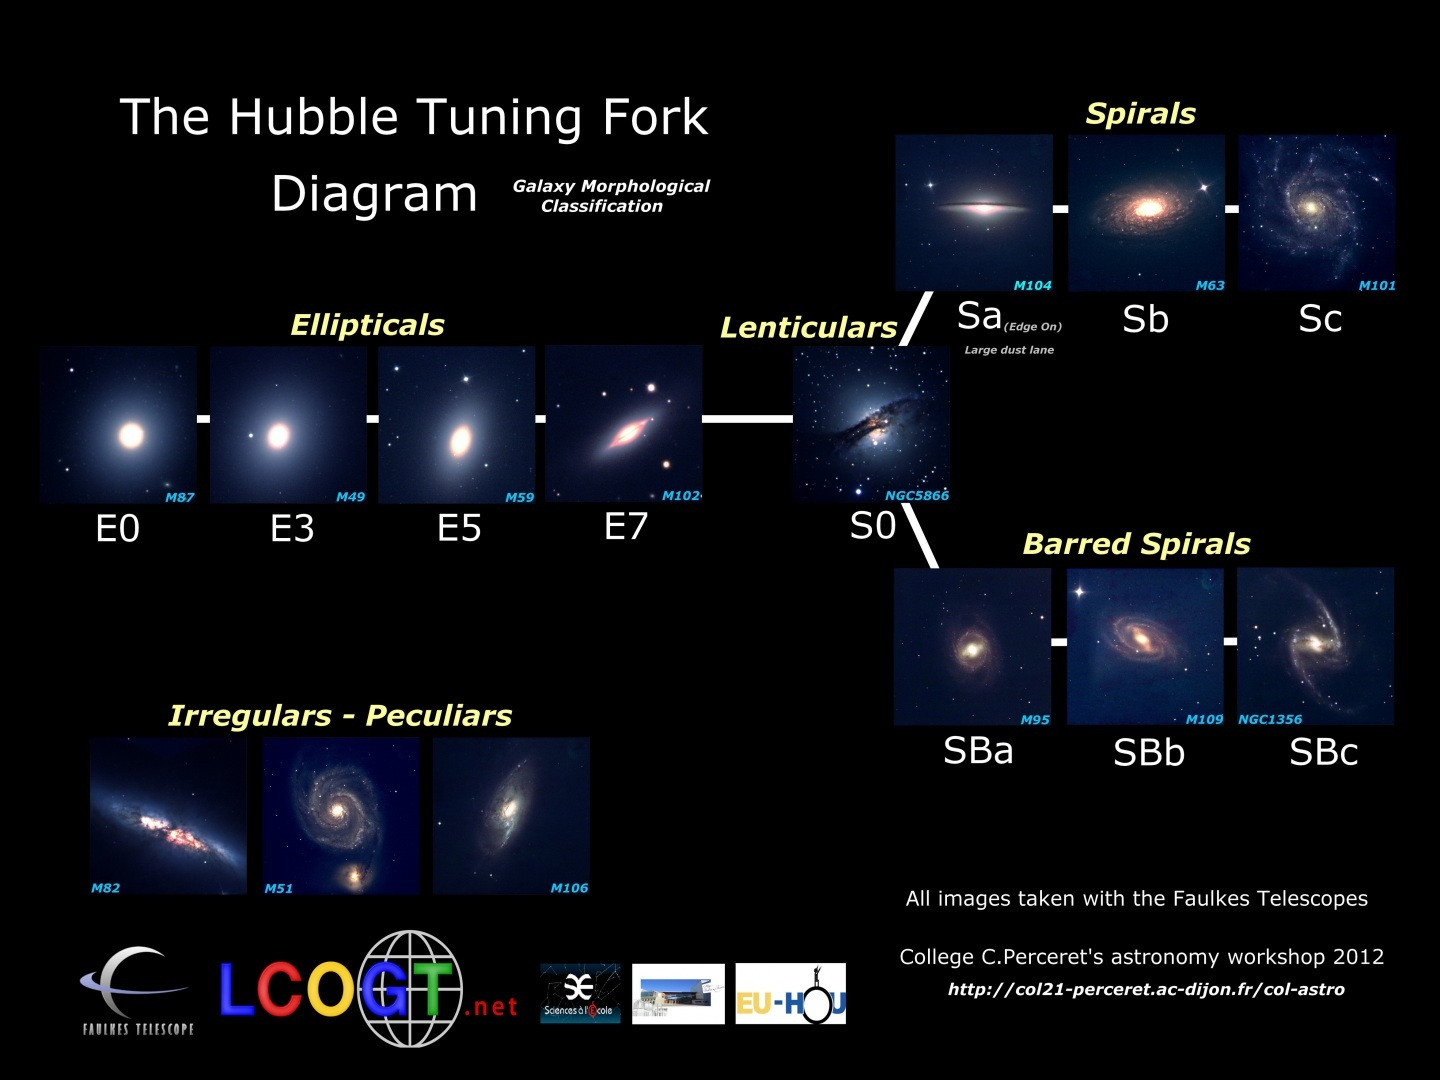
\includegraphics[width=\textwidth]{introduction/hubble-tuning-fork-diagram}
\caption{The Hubble sequence demonstrated graphically as the Hubble Tuning Fork from \cite{hubble_tuning_fork} . This diagram illustrates Hubble's classification of galaxies by their morphologies into ellipticals, spirals, lenticulars, and irregulars.}
\label{fig:hubble_tuning_fork}
\end{figure*}

% In Hubble's work, the galaxies employed were bright, local objects with total magnitudes ranging from $m_T\sim$9--13 and redshifts $z\approx0$. With data only representing the local universe, there is no clear indication on whether the Hubble sequence is applicable to the history and future of galactic evolution. 
% the above paragraph is alluding to my project, I don't think it's needed here just yet

Subsequent identification schemes would refine and build on the Hubble sequence as larger datasets became more readily available. These would contain a greater variety of extra-galactic objects and allow for arguments such as expanding the spiral category due to the importance of rings and lenses as their defining features \citep{1959HDP....53..275D}. 

Through Hubble's work, galaxies can be comprehensively classified by their morphologies, however these do not fully reflect the internal content of a galaxy. For an indicator of the inner dynamics, fundamental parameters should be employed in tandem with the morphological classification. 

\vspace{2ex}
\subsection{Dynamical studies of galaxies along the Hubble sequence}
\subsubsection{Angular momentum and the evolution of galactic dynamics}
\noindent
The mass, energy, and angular momentum are three physical values which can be used as a quantitative classification of a galaxy. 

The angular momentum is of particular interest as the defining morphologies of a galaxy is most likely a result of the primeval mass--angular momentum distribution \citep{1970ApJ...160..831S}. The acquisition of this angular momentum in a protogalactic system has been proposed to be a result of the tidal interactions with nearby early protogalaxies \citep{1969ApJ...155..393P}. Within a young spiral system, these tidal torques induce galactic spin and lead to massive extended haloes if discs within spirals have radii comparable to those observed in the present day. By extension, the dynamics of these spiral discs and their stellar populations can be modelled to demonstrate that the present day observed sizes and rotation velocities are consistent with the conservation of the early angular momentum \citep{1998MNRAS.295..319M, 1997ApJ...482..659D}. 

Measurements of the angular momentum for a galaxy can be employed to reconstruct the initial formation conditions present within the protogalaxy, and by extension predict the potential evolution for the galaxy. 

% what does the Romanowsky and Fall plot show?
% the plot itself shows the relationship between stellar specific angular momentum and stellar mass for various types of galaxies - how is this important? 
% it's the slow building up to scaling relations which I should provide some info on here, in this section - next section is a discussion of Tully-Fisher and Faber-Jackson

Obtaining the stellar specific angular momentum $j_*$ and the stellar mass $M_*$ within a galaxy, a 

\begin{figure}
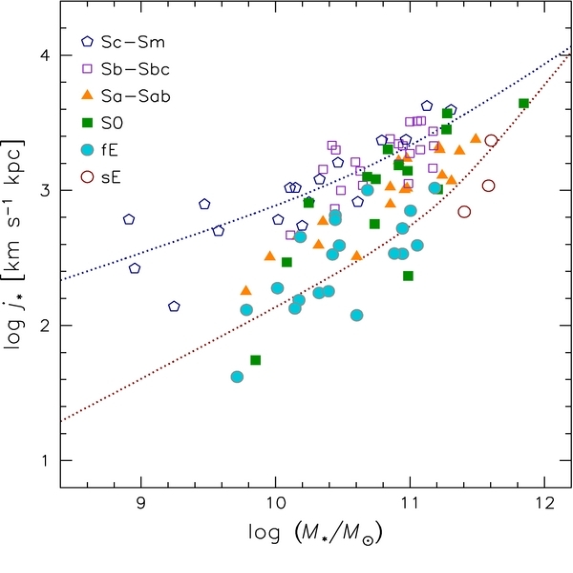
\includegraphics[width=1.0\linewidth]{introduction/romanowsky_2012_fig_3}
\captionsetup{justification=raggedright}
\caption{The stellar specific angular momentum and stellar mass relationship for spiral and elliptical galaxies from \cite{2012ApJS..203...17R}. A galaxy's angular momentum is indicative of how it formed and the type of morphology it possess.}
\label{fig:romanowsky_fall_2012}
\end{figure}

% could expand on the figure caption

\vspace{4ex}
\subsubsection{Tully-Fisher and Faber-Jackson relationships}

% show plots of the TF and FB relationships from their original papers and then discuss how they are useful
% they are relationships for spirals and elliptical galaxies which detail what??
% discuss how these relations are derived at the local universe i.e. using data at z~0

\subsection{High-redshifts}

\subsubsection{Galaxy formation models}

for such as N-body interactions in large-scale galaxy cluster structures or 

% Dynamical constraints
% Galaxy formation models through EAGLE and TFR
% discuss how to understand the formation and evolution of galaxies one method is to simulate them
% This simulates the galaxy in a hollisitic approach

\subsubsection{Stellar formation}

% Madau plot with stellar formation 
% formation of stars is linked to the formation of the galaxy
% Any future relationship between stars and other components of the galaxy is linked i.e. the gas

\subsubsection{Evolution of scaling relations}

% evolution of dark matter haloes

\subsection{The Hubble Ultra Deep Field}

\subsubsection{HST}

% I don't want to later repeat myself later in the second section - I want to provide some basic history for HST and for MUSE
% How about a discussion on what the instruments are and then later on in the observations section I should be discussing the exact specifics on how the data was obtained
% Maybe I can provide the basic schematics 
% What can optical data tell us e.g. colour images, morphology...etc

\begin{figure*}
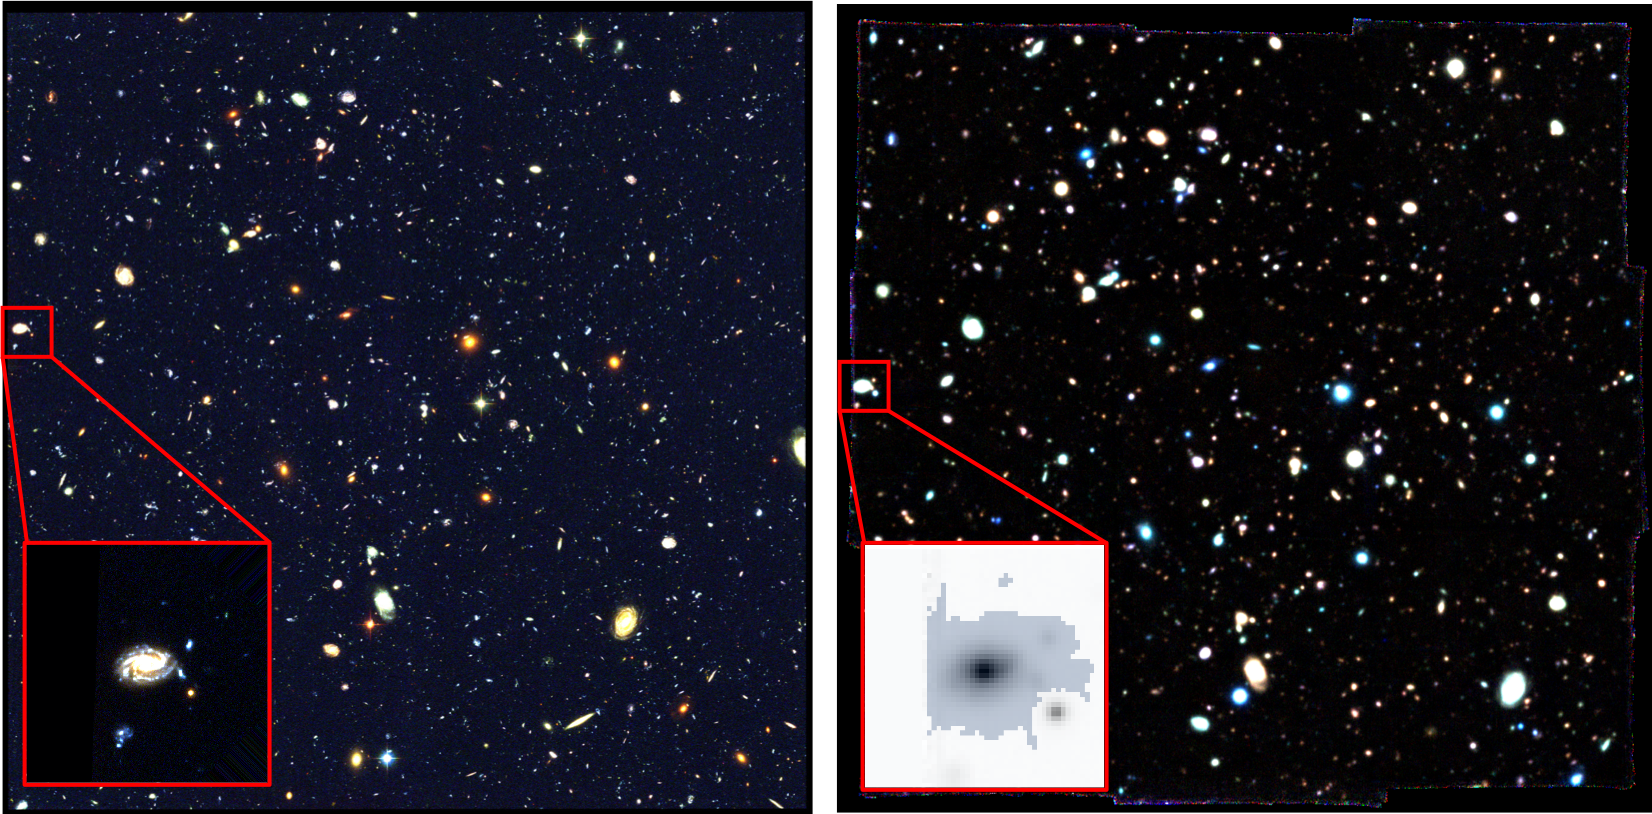
\includegraphics[width=\textwidth]{introduction/hudf_frame.pdf}
\captionsetup{justification=justified, format=plain}
\caption[Hubble Ultra Deep Field]{\textit{Left-hand panel}: colour composite image for the HUDF from HST ACS/WFC, Hubble eXtreme Deep Field project data \citep{2013ApJS..209....6I}. Frames in three filter bands (F775W, F606W, and F435W) were combined to represent the RGB channels within a colour image. \textit{Right-hand panel}: colour image of the MUSE HUDF region. The spectra wavelength range (4650 \AA--9300 \AA) of the MUSE cube was divided into three equal regions (4650 \AA--6180 \AA, 6180 \AA--7730 \AA, 7730 \AA -- 9300 \AA), collapsed, and then combined to create an RGB image. Highlighted in both images is object RAF-24420 \citep{2015AJ....150...31R}, the HST data has a higher optical resolution whereas the MUSE data outclasses in the resolution of the spectroscopic data.}
\label{fig:hst_muse_hdf}
\end{figure*}

\subsubsection{MUSE}

% Redshifts
% Dynamics
% Velocity dispersions of stars and gas
% Stellar populations: IMF
% Stellar metallicity Z

\begin{table}
\begin{center}
\begin{tabular}{c@{\hskip 20pt}c} 
 \hline
 \textbf{Type} & \textbf{Colour and notable lines} \\ [0.5ex] 
 O & Hot blue-white (HeII, HeI) \\
 B & Hot blue-white (HeI, HI ) \\
 A & White (Balmer, CaII) \\
 F & Yellow-white (CaII, FeI, Cr,I) \\
 G & Yellow (CaII, FeI,  \\
  & neutral metals) \\
 K & Cool orange (CaII H and \\ 
  & K, metals) \\
 M & Cool red (TiO, VO, neutral \\
  & metals) \\
 L & Very cool, dark red, infrared \\
  & (Molecular absorption, CrH, \\
  & FeH, H$_2$O, CO, Na, K, Rb, Cs) \\
 T & Coolest, infrared (CH$_4$, CO) \\
 \hline
\end{tabular}
\caption{The Harvard Spectral Classification for stellar objects \citep{1916AnHar..76...19C}. Stars are defined by their colour (temperature) and features seen from their spectra \citep{stellar_colour, 1925PhDT.........1P}. Provided are spectral types, and their associated colour plus the main emission or absorption lines. Figure \ref{fig:spectral_types} provides examples of the possible observed spectra for spectral types \textit{OBAFGKM}.}
\label{table:spectral_classification}
\end{center}
\end{table}

\begin{figure*}
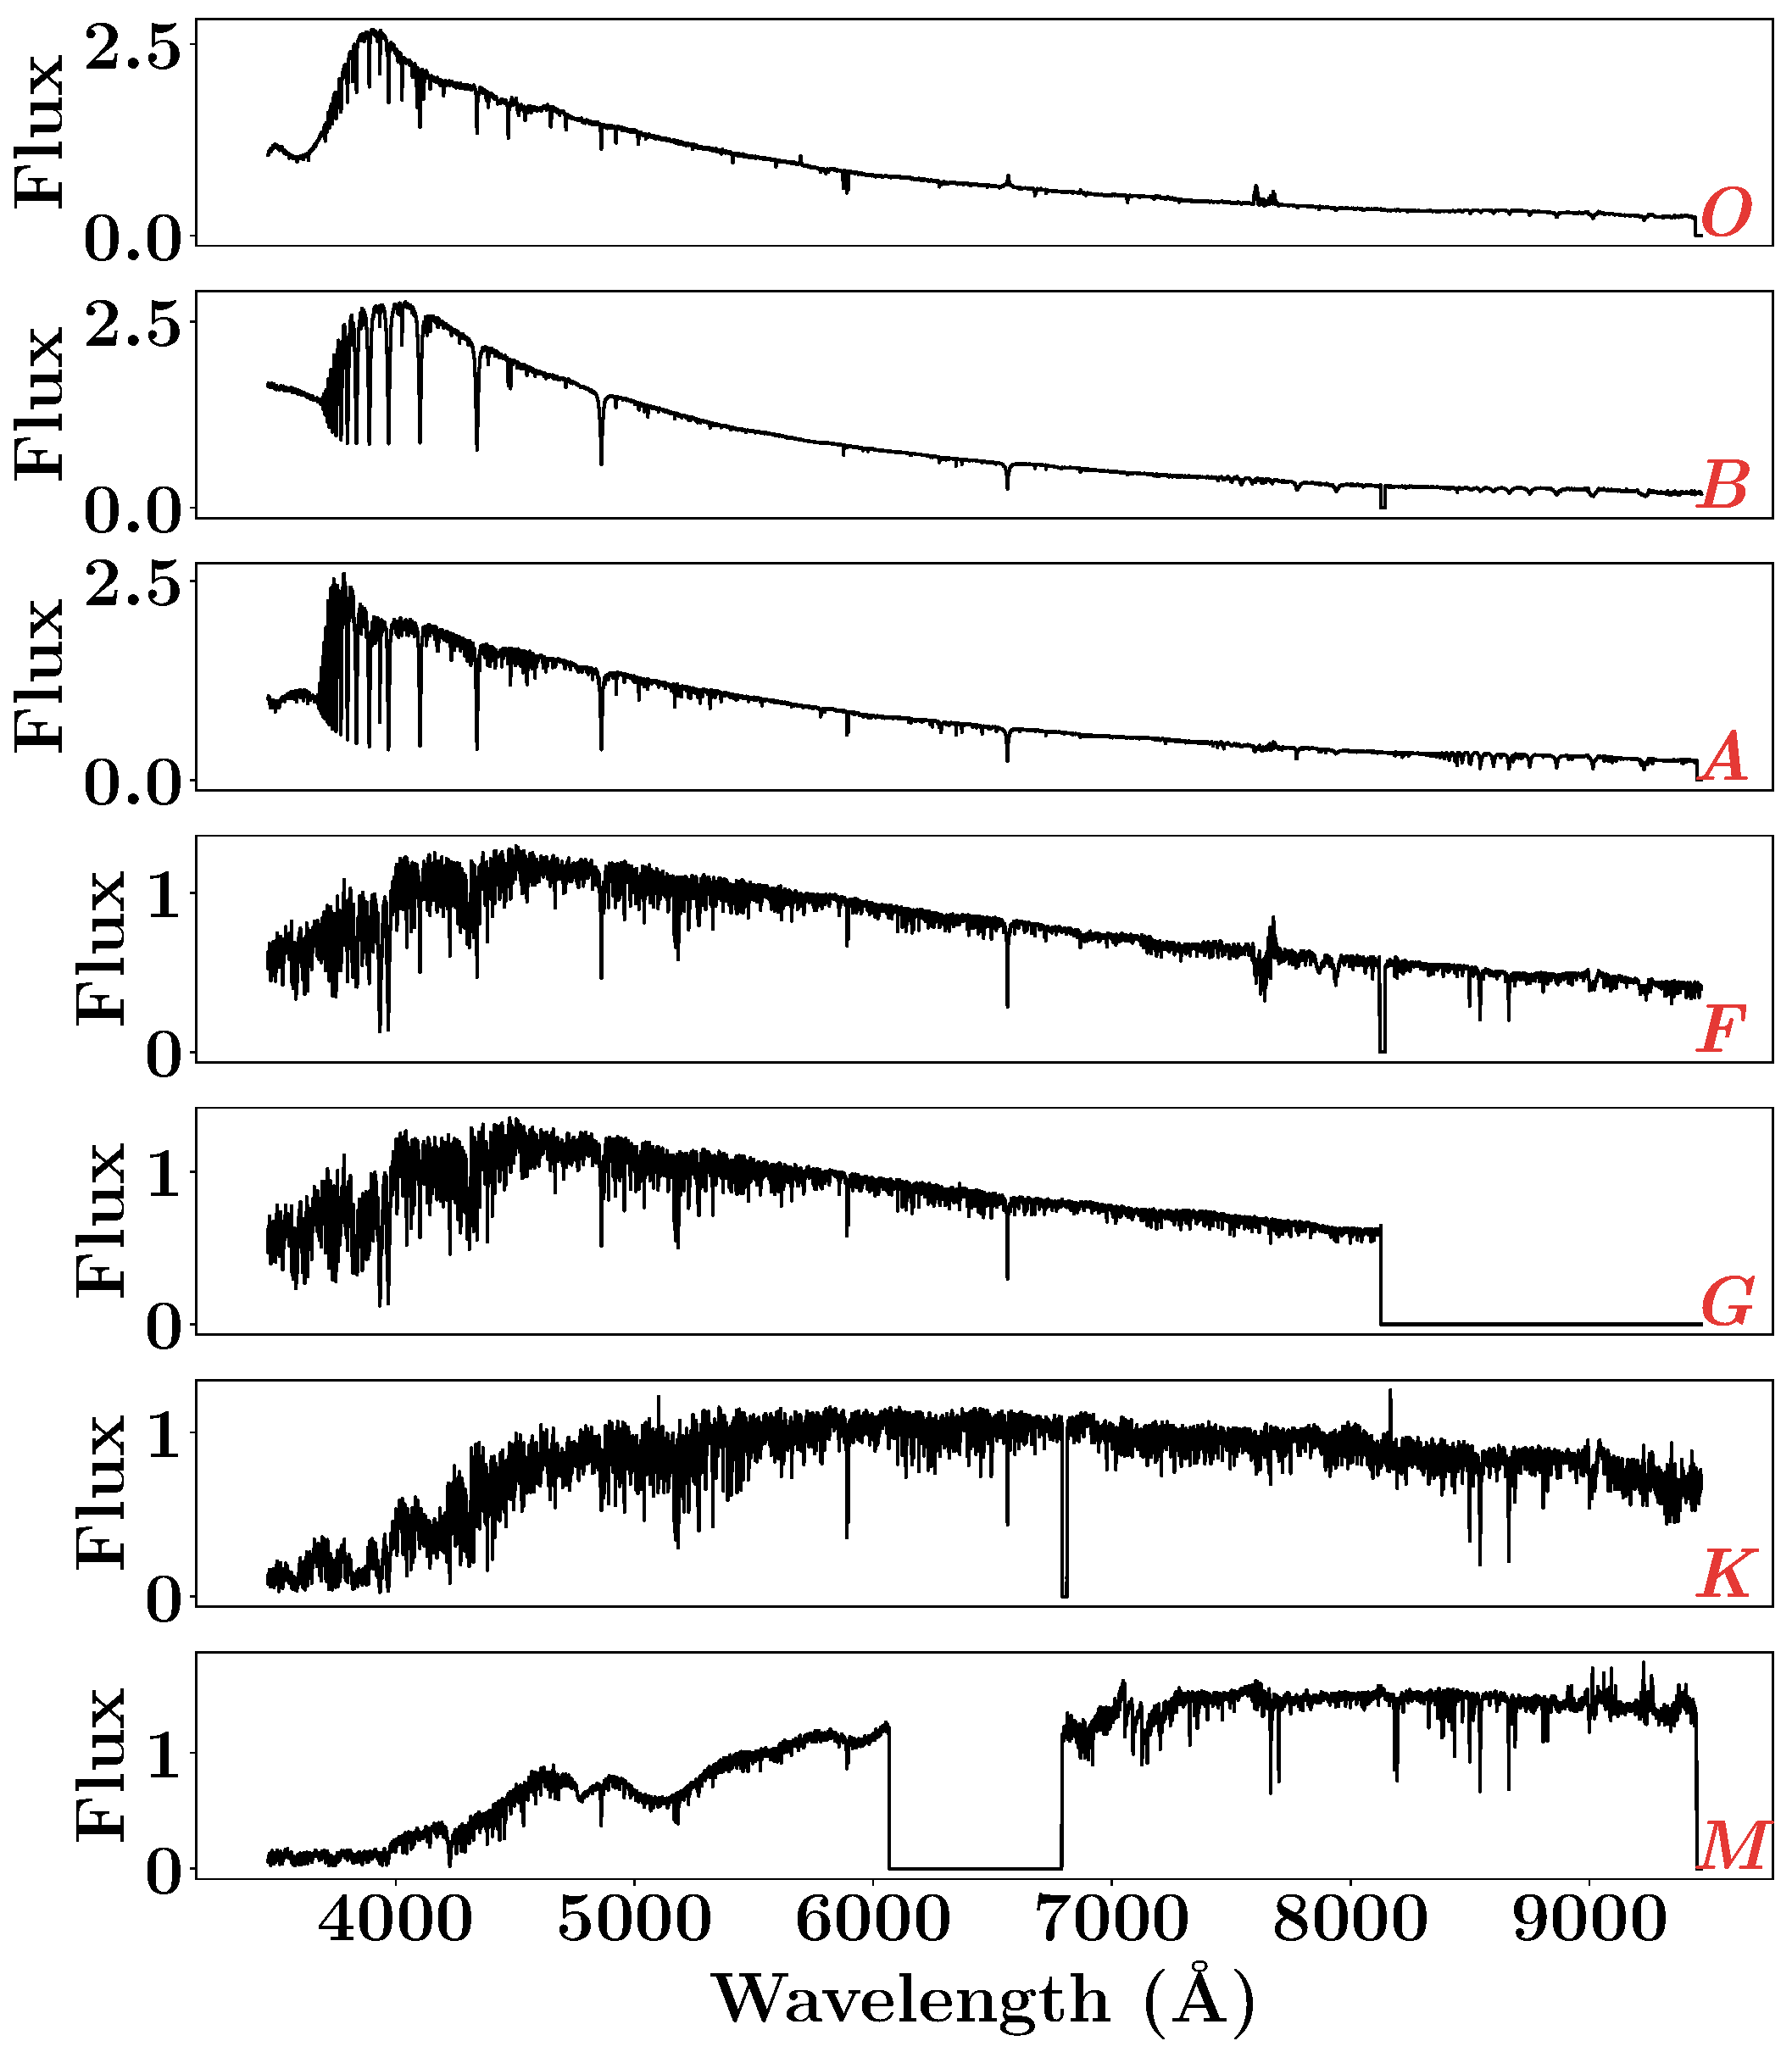
\includegraphics[width=1.0\linewidth]{introduction/spectral_types}
\caption{Example spectra for spectral types \textit{OBAFGKM}. Taken from the Indo-US Library of Coudé Feed Stellar Spectra \citep{valdes_coude}, the stars used have metallicities [Fe/H]$_{\odot} \approx0$  and are: 30614 (\textit{O}), 17081 (\textit{B}), 39866 (\textit{A}), 5015 (\textit{F}), G 7-6 (\textit{G}), 5858 (\textit{K}), and G 176-11 (\textit{M}). These spectra demonstrate that older types (\textit{FGKM}) have larger amounts of absorption and emission lines when compared to younger types (\textit{OBA}) as they have spent a greater amount of time undergoing nuclear fusion. Galaxy spectra will contain combinations of these stars which produces a unique profile.}
\label{fig:spectral_types}
\end{figure*}

\subsection{Project study and aims} % think of a better heading for this

% Linking between the gas and stars at high redshift to test the scaling relations 
% Is OII a valid and applicable method in testing the scaling relations

This paper discusses the study undertaken to understand the dynamics between the gas and stars in galaxies. Data extraction is performed on a MUSE data cube, the sample is reduced, and various fittings are then applied to the dataset.

In Section \ref{sec:analysis}, the methodology of galaxy extraction from the MUSE cube is discussed, as well as the subsequent analysis performed by applying different fitting routines: [OII] Gaussian doublet fittings, and fitting with a penalised pixel-fitting method. 

\section{Observations and data analysis}

\subsection{HST HUDF}

\subsection{MUSE HUDF}
\noindent

\begin{figure}
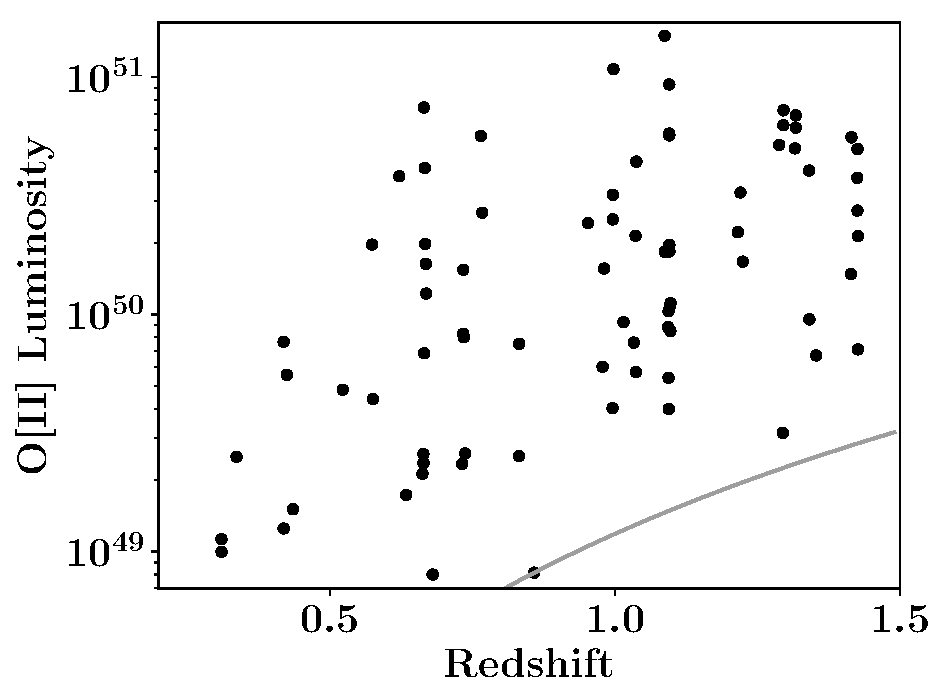
\includegraphics[width=1.0\linewidth]{data/o_ii_luminosity_vs_redshift}
\caption{[OII] luminosity against redshift for 84 galaxies. Lower-limit of this sample (grey) was calculated using the object with the smallest flux. All galaxies appear above this limit and approximately follow the luminosity-redshift trend. Note that objects with $z<0.3$ were not analysed as high-redshift galaxies were desired. }
\label{fig:oiiluminosity_redshift}
\end{figure} 

% Variables used for each galaxy were obtained from the fitting of the galaxy-integrated spectra with a model (Equation \ref{eqn:doublet})

After performing the sample reduction methods the final objects shown as \textit{Usable} in Figure \ref{fig:sn_vband} can be found in Table [reference].

\begin{figure*}
  \subfloat{\label{fig:image_sn_vband}%
  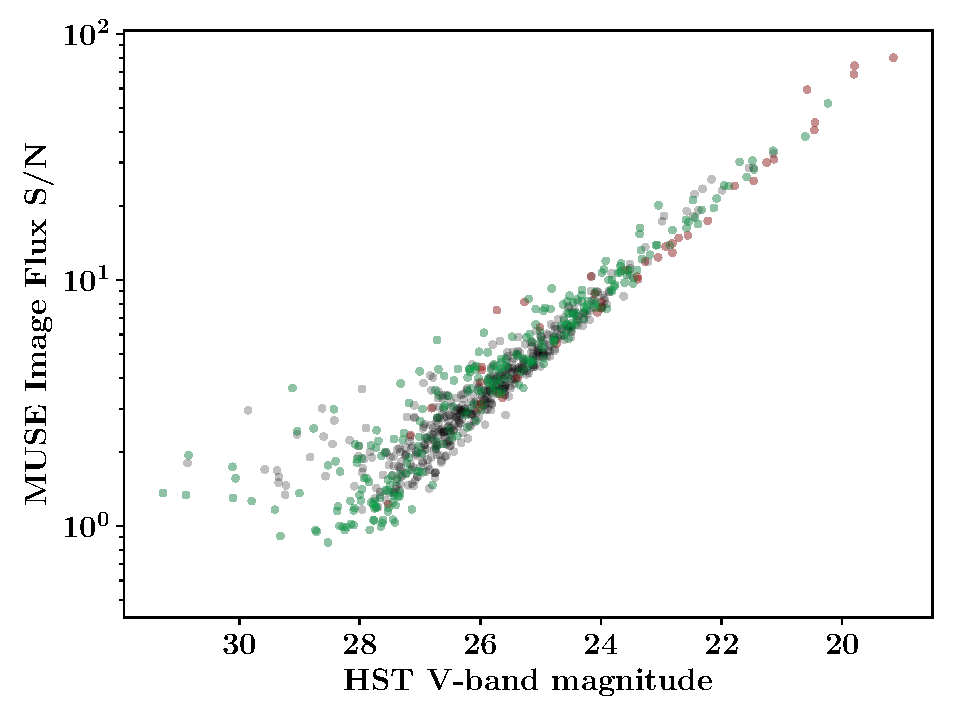
\includegraphics[width=0.5\textwidth]{data/image_sn_vs_vband}%
  }
  %
  \subfloat{\label{fig:spec_sn_vband}%
  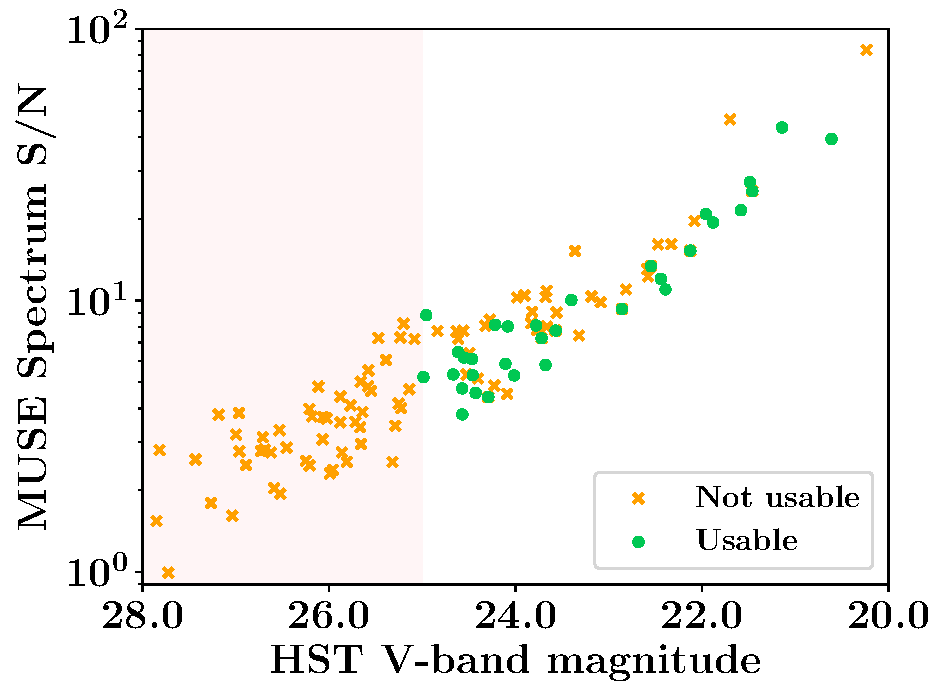
\includegraphics[width=0.5\textwidth]{data/sn_vs_vband}%
  }
  \captionsetup{justification=raggedright}
  \caption[HUDF Objects]{\textit{Left-hand panel}: MUSE image flux signal-to-noise (S/N) versus HST V-band magnitude for the first 300/837 extracted cubes which were ranked by redshift $z$. \textit{Right-hand panel}: MUSE spectrum signal-to-noise (S/N) versus HST V-band magnitude for reduced sample of extracted objects. \textit{Both}: the red area indicates an imposed magnitude limit of 25.0 mag. The reduction of the cubes to produce the final sample was highly dependent on whether an object was actually a galaxy, if an [OII] feature was present, and whether there was enough S/N for visible absorption features. This gave rise to the ``Not usable'' classification as shown. From the total sample of 837 objects, this was reduced down to 35 potentially usable galaxies.}
\label{fig:sn_vband}
\end{figure*}

% Image flux and noise was obtained during the extraction of galaxies from the MUSE 3D cube. 
% Spectrum S/N was calculated with the median and standard deviation of the region $3700\times(1+z)$ {\AA} to $4500\times(1+z)$ {\AA} in the galaxy integrated spectra, with $z$ as the redshift.
% From a total sample of 837 objects, 300 were
% Objects were sorted by their probability in being a star and an initial analysis performed down to 31.0 mag to check if they contained an [OII] feature. ``Unused'' extractedclassed as unused if they had a $>60\%$ probability

\onecolumngrid

\begin{sidewaystable*}
\centering
\begin{tabular}{c@{\hskip 10pt}c@{\hskip 10pt}c@{\hskip 10pt}c@{\hskip 10pt}c@{\hskip 10pt}c@{\hskip 10pt}c@{\hskip 10pt}c@{\hskip 10pt}c@{\hskip 10pt}c} 
 \hline
 \textbf{Cube ID} & \textbf{RAF ID} & \textbf{RA (deg)} & \textbf{Dec. (deg)} & \textbf{F606W mag.} & \textbf{$\boldsymbol{z}$} & \textbf{$\boldsymbol{V_*}$ (kms$^{-1}$)} & \textbf{$\boldsymbol{\sigma_*}$ (kms$^{-1}$)} & \textbf{$\boldsymbol{V_{OII}}$ (kms$^{-1}$)} & \textbf{$\boldsymbol{\sigma_{OII}}$ (kms$^{-1}$)} \\ [0.5ex] 
C1804 & 24420 & 53.1783773 & -27.76824447 & $21.4864(8)$ & $0.66850(6)$ & $153531(10)$ & $182(25)$ & $153471(24)$ & $ 147(35)$ \\ 

C1578 & 22735 & 53.13064889 & -27.79026088 & $21.880(1)$ & $0.66640(5)$ & $153185(7)$ & $117(12)$ & $153094(18)$ & $ 139(25)$ \\ 

C849 & 21651 & 53.17251203 & -27.79636076 & $22.125(1)$ & $0.347053(5)$ & $89414(8)$ & $3.8(7)$ & $89314(18)$ & $ 79(24)$ \\ 

C286 & 24587 & 53.16992265 & -27.77102451 & $21.1412(9)$ & $0.62169(1)$ & $145050(7)$ & $58(6)$ & $144939(17)$ & $ 91(16)$ \\ 

C5 & 20595 & 53.15639984 & -27.81081513 & $21.5823(8)$ & $0.66459(2)$ & $152807(9)$ & $78(10)$ & $152768(21)$ & $ 110(24)$ \\ 

C767 & 21364 & 53.18023505 & -27.79892259 & $21.958(1)$ & $0.6673(1)$ & $153328(10)$ & $148(21)$ & $153250(24)$ & $ 141(34)$ \\ 

C414 & 7253 & 53.15153909 & -27.76201929 & $22.546(3)$ & $0.42451(5)$ & $106177(10)$ & $106(21)$ & $106076(23)$ & $ 128(42)$ \\ 

C549 & 24515 & 53.15256871 & -27.76950996 & $22.858(3)$ & $0.33644(1)$ & $87049(9)$ & $25(6)$ & $86943(22)$ & $ 85(32)$ \\ 

C175 & 8246 & 53.18480046 & -27.77745246 & $23.570(4)$ & $0.52255(2)$ & $126111(11)$ & $127(25)$ & $126029(28)$ & $ 82(28)$ \\ 

C1129 & 9958 & 53.13928756 & -27.78066897 & $23.677(4)$ & $0.73403(2)$ & $165114(19)$ & $60(15)$ & $165020(46)$ & $ 95(41)$ \\ 

C765 & 23794 & 53.15817553 & -27.78109416 & $22.391(2)$ & $0.619373(2)$ & $144615(12)$ & $65(12)$ & $144512(30)$ & $ 64(20)$ \\ 

C1075 & 3630 & 53.16129898 & -27.79547518 & $23.720(3)$ & $0.30988(3)$ & $80989(11)$ & $143(41)$ & $80925(26)$ & $ 77(38)$ \\ 

C540 & 24348 & 53.16236468 & -27.77506443 & $21.4602(8)$ & $0.41894(2)$ & $105015(8)$ & $60(10)$ & $104899(19)$ & $ 91(25)$ \\ 

C895 & 39778 & 53.14168389 & -27.77310068 & $24.291(6)$ & $0.52461(2)$ & $126561(18)$ & $0.5(2)$ & $126434(43)$ & $ 73(38)$ \\ 

C554 & 38260 & 53.14916378 & -27.76363345 & $23.401(3)$ & $0.737184(4)$ & $165687(12)$ & $123(20)$ & $165565(30)$ & $ 70(19)$ \\

C109 & 9475 & 53.18591136 & -27.77561507 & $24.084(4)$ & $1.42553(8)$ & - & - & - & - \\ 

C310 & 8531 & 53.16632928 & -27.76858816 & $23.778(5)$ & $1.29533(2)$ & - & - & - & - \\ 

C363 & 8672 & 53.16395412 & -27.76905273 & $24.569(7)$ & $0.41891(3)$ & - & - & - & - \\ 

C486 & 51705 & 53.18782913 & -27.79405589 & $20.6113(5)$ & $0.345393(8)$ & - & - & - & - \\ 

C254 & 4686 & 53.19373778 & -27.78787018 & $24.572(7)$ & $0.43534(3)$ & - & - & - & - \\ 

C688 & 5773 & 53.17805845 & -27.79274792 & $25.82(2)$ & $1.4263(1)$ & - & - & - & - \\ 

C759 & 8949 & 53.14617923 & -27.77103939 & $24.108(5)$ & $1.3155(2)$ & - & - & - & - \\ 

C1394 & 2908 & 53.1525505 & -27.80037599 & $24.99(1)$ & $1.4254(1)$ & - & - & - & - \\ 

C847 & 21703 & 53.17365111 & -27.7973635 & $24.218(5)$ & $0.66543(1)$ & - & - & - & - \\ 

C1665 & 50714 & 53.15110943 & -27.80949195 & $24.552(4)$ & $1.08753(3)$ & - & - & - & - \\ 

C541 & 24353 & 53.16081556 & -27.77537746 & $22.442(2)$ & $0.62149(6)$ & - & - & - & - \\ 
 \hline
\end{tabular}
\caption{Parameters for the final reduced sample of 35 galaxies. Columns show the working cube ID, the ID from the UVUDF Catalogs \citep{2015AJ....150...31R} (RAF ID), the object right ascension (RA) and declination (Dec.), the magnitude of the object in the HST F606W filter, the calculated galaxy redshift ($z$), the galaxy stellar velocity ($V_*$) and velocity dispersion ($\sigma_*$), and the galaxy gas velocity ($V_{OII}$) and velocity dispersion ($\sigma_{OII}$. Note that only 15 galaxies were analysed for their stellar and gas components as the majority of the sample contained spectra with not enough signal-to-noise. 11 of the non-analysed galaxies are provided here with the rest contained in Appendix \ref{appendix:rest_of_final_sample}.}
\label{table:final_sample}
\end{sidewaystable*}

\twocolumngrid

\section{Discussion}

\subsection{Galaxy velocity dispersions}

\subsubsection{[OII] modelling}

\subsubsection{Full spectrum modelling}

\subsubsection{$\sigma$ results}

\begin{figure*}
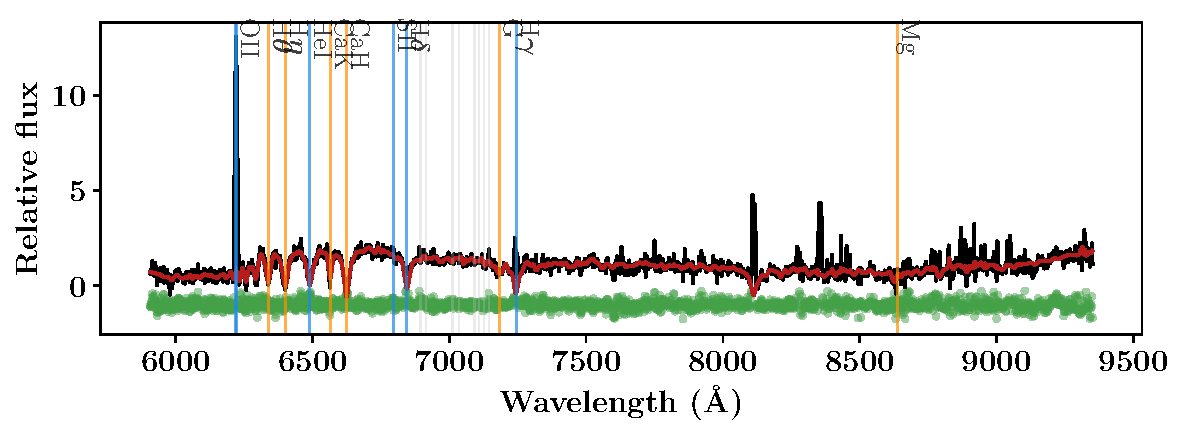
\includegraphics[width=\textwidth]{data/cube_1804_spectra_complete}
\caption{Example spectra and the pPXF analysis performed for C1804. The galaxy integrated spectra (black) would be passed to the pPXF fitting routine which would normalise the data and return a best fitting model (red) plus values for galaxy velocity and velocity dispersion. The residuals between the data and model (green) are shown in addition to some highlighted emission (blue), absorption (orange), and iron (grey) spectra features. For C1804 in particular, pPXF provided a reduced $\chi^2 \approx 1.69$ which is an indication of a good fit.}
\label{fig:ppxf_spectra}
\end{figure*}

\begin{figure}
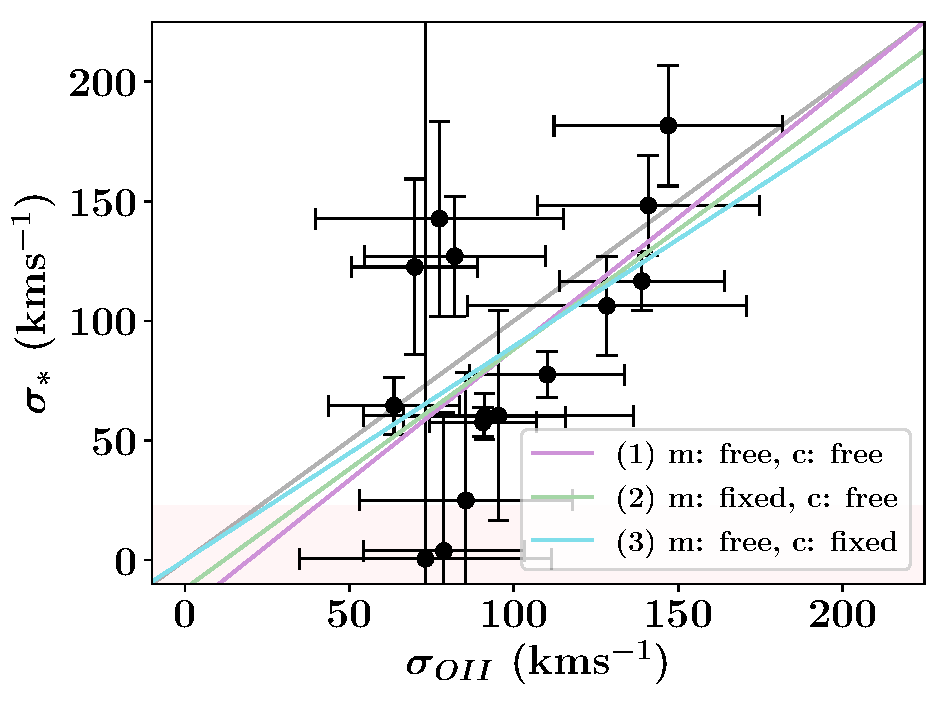
\includegraphics[width=1.0\linewidth]{data/sigma_star_vs_sigma_oii}
\caption{Stellar velocity dispersions ($\sigma_*$) versus [OII] gas velocity dispersions ($\sigma_{OII}$) for a sample of 15 galaxies. Three linear models were fitted to the data: (1) free gradient and free intercept, $\chi^2_{\nu}=9.43$; (2) fixed gradient and free intercept, $\chi^2_\nu=9.62$; and (3) free gradient and fixed intercept, $\chi^2_\nu=5.87$. Model 3 is the best fit, and from the data a linear model appears to be the best consideration. $\sigma_*$ values are limited by the instrumental resolution of MUSE and values within this range ($<\sigma_{inst}/2=22.7$ kms$^{-1}$) should be considered with caution.  }
\label{fig:velocity_dispersions}
\end{figure}

\begin{figure*}
\centering
\subfloat{\label{fig:ppxf_sigma_frac_error_vs_sn}%
  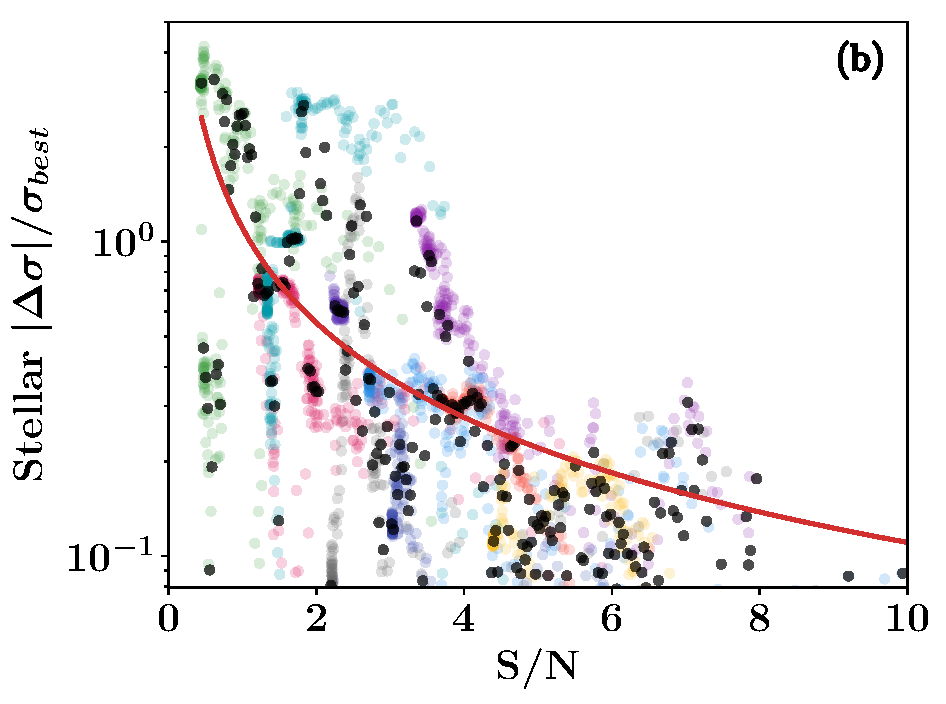
\includegraphics[width=0.495\textwidth]{data/ppxf_sigma_frac_error_vs_sn}%
  }
\subfloat{\label{fig:lmfit_sigma_frac_error_vs_sn}%
  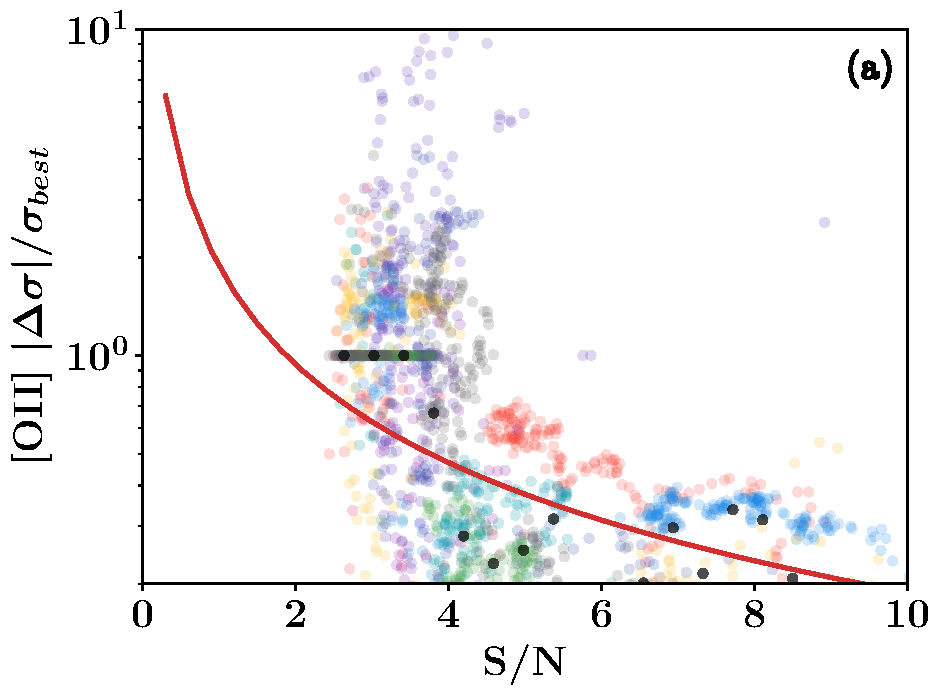
\includegraphics[width=0.495\textwidth]{data/lmfit_sigma_frac_error_vs_sn}%
  }\\
\subfloat{\label{fig:ppxf_vel_frac_error_vs_sn}%
  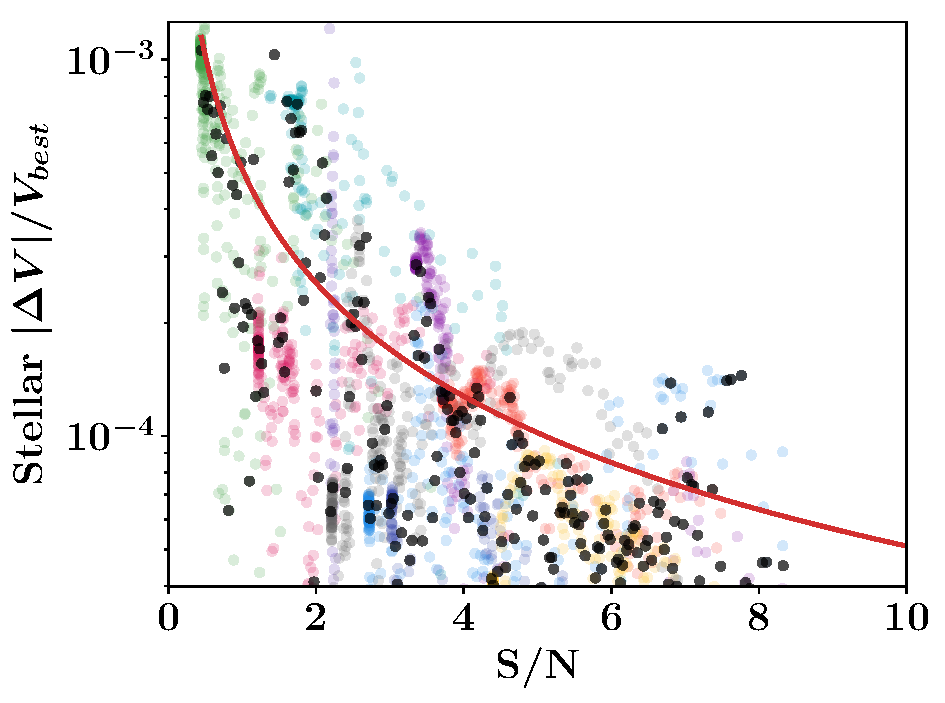
\includegraphics[width=0.495\textwidth]{data/ppxf_vel_frac_error_vs_sn}%
  }
\subfloat{\label{fig:lmfit_vel_frac_error_vs_sn}%
  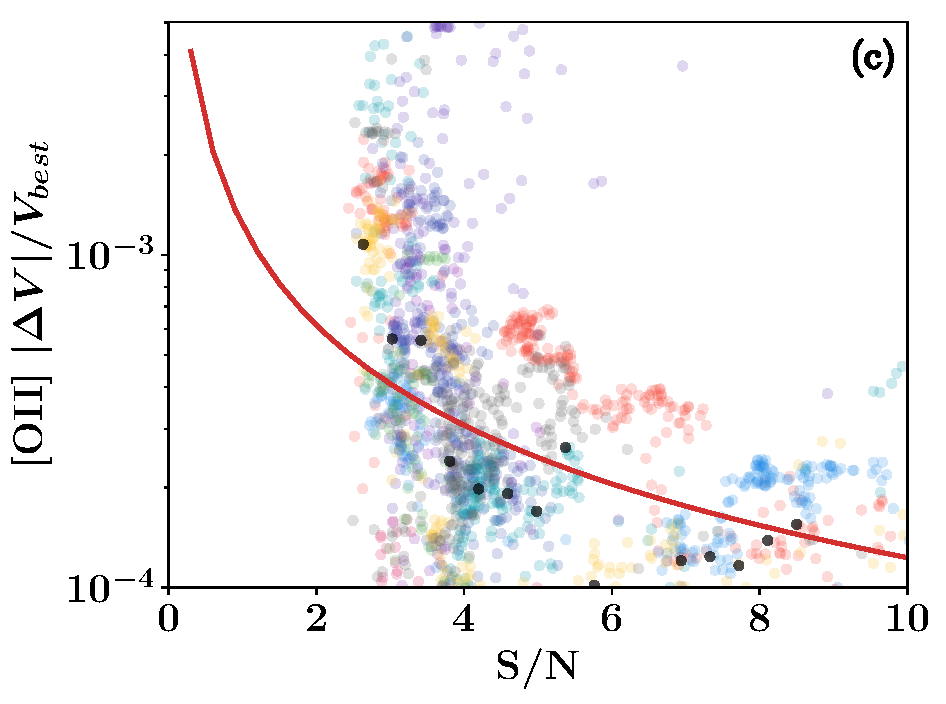
\includegraphics[width=0.495\textwidth]{data/lmfit_vel_frac_error_vs_sn}%
  }
\captionsetup{justification=raggedright}
\caption[HUDF Objects]{\textit{Top panel}: fractional error versus signal-to-noise for stellar and [OII] gas velocity dispersions. \textit{Bottom panel}: fractional error versus signal-to-noise for the stellar and [OII] gas velocities. \textit{All}: the $a/x$ models (red) provided alternative uncertainties on acquired $V$ and $\sigma$ values. The fitting routines would produce their own errors but their reliability was questioned and their methodology unknown.}
  \label{fig:fractional_errors}
\end{figure*}

% the spectra for the 15 usable galaxies were sequentially perturbed with normal noise, fitted with [OII] and absorption models, fractional difference calculated between 

% a polynomial $a/x$ model was fitted to all four data sets. As the S/N decreases, the difference increases manifold which implies that high S/N galaxies should be used as they would have smaller fractional uncertainty.

%\subsubsection{Old vs. new stellar types}

\begin{figure}
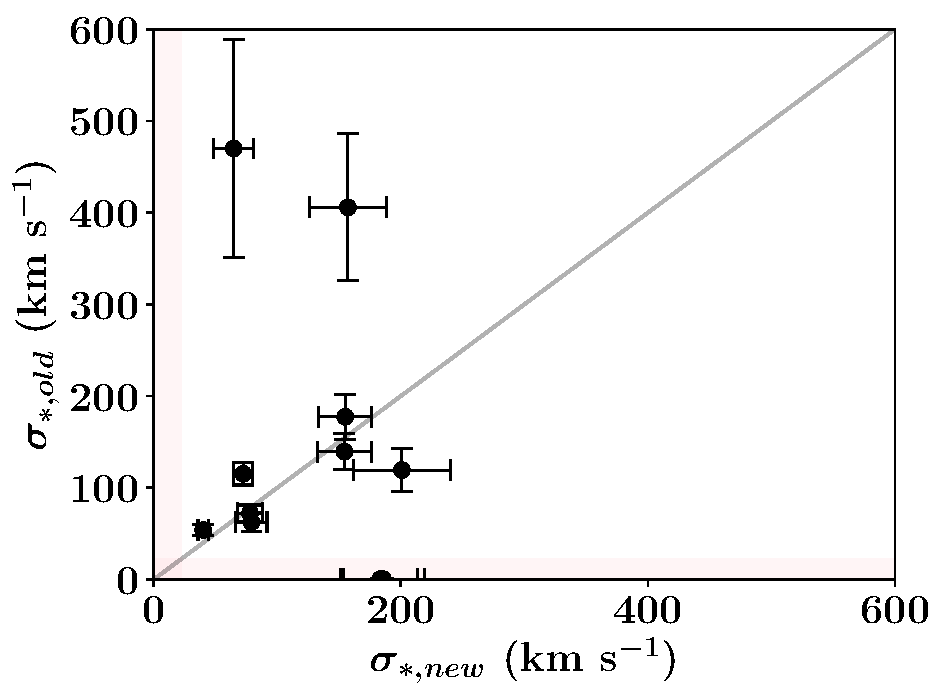
\includegraphics[width=1.0\linewidth]{data/sigma_stars_old_vs_new}
\caption{Velocity dispersions for old stellar types (\textit{GK}) versus those for new (young) stellar types (\textit{OA}). 11 galaxy spectra were isolated into overlapping regions of $3700\times (1+z)$ {\AA} to $4200\times(1+z)$ {\AA} for young stars, and $4000\times (1+z)$ {\AA} to $4500\times(1+z)$ {\AA} for old stars. If a linear trend is considered then two spiral galaxies (C1129 and C175) strongly deviate from this line. This could be attributed to the difficulty in fitting for smaller wavelength regions or to problems with high noise. }
\label{fig:velocity_dispersions_old_new}
\end{figure} 

% produce a chi^2 value for the above relationship

\subsection{Galaxy velocities}

%\subsubsection{$V_{*}$ vs. $V_{OII}$}

\begin{figure}
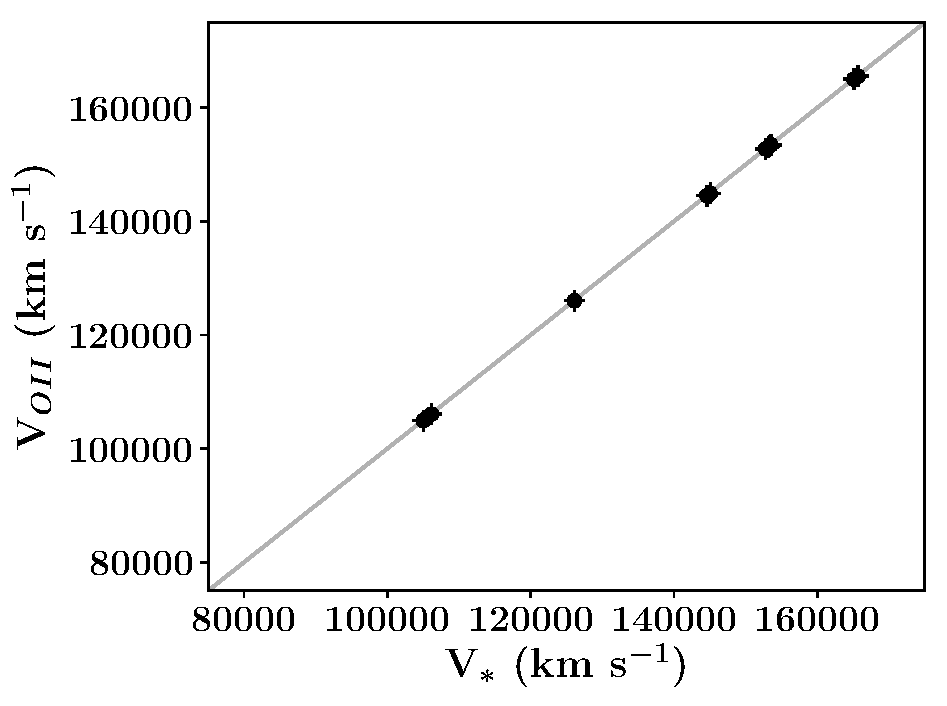
\includegraphics[width=1.0\linewidth]{data/vel_star_vs_vel_oii}
\caption{Stellar and [OII] gas velocities for 15 galaxies. The calculated velocities appear to be well in agreement with each other with a $0.0757\%$ fractional difference. It would be expected that both components move at the same relative velocity.}
\label{fig:velocities}
\end{figure}

% By appearance the calculated velocities appear to be well in agreement with each other.

\subsection{Voronoi tessellation}

\subsubsection{Tully-Fisher}

\onecolumngrid

\begin{sidewaysfigure*}
\centering
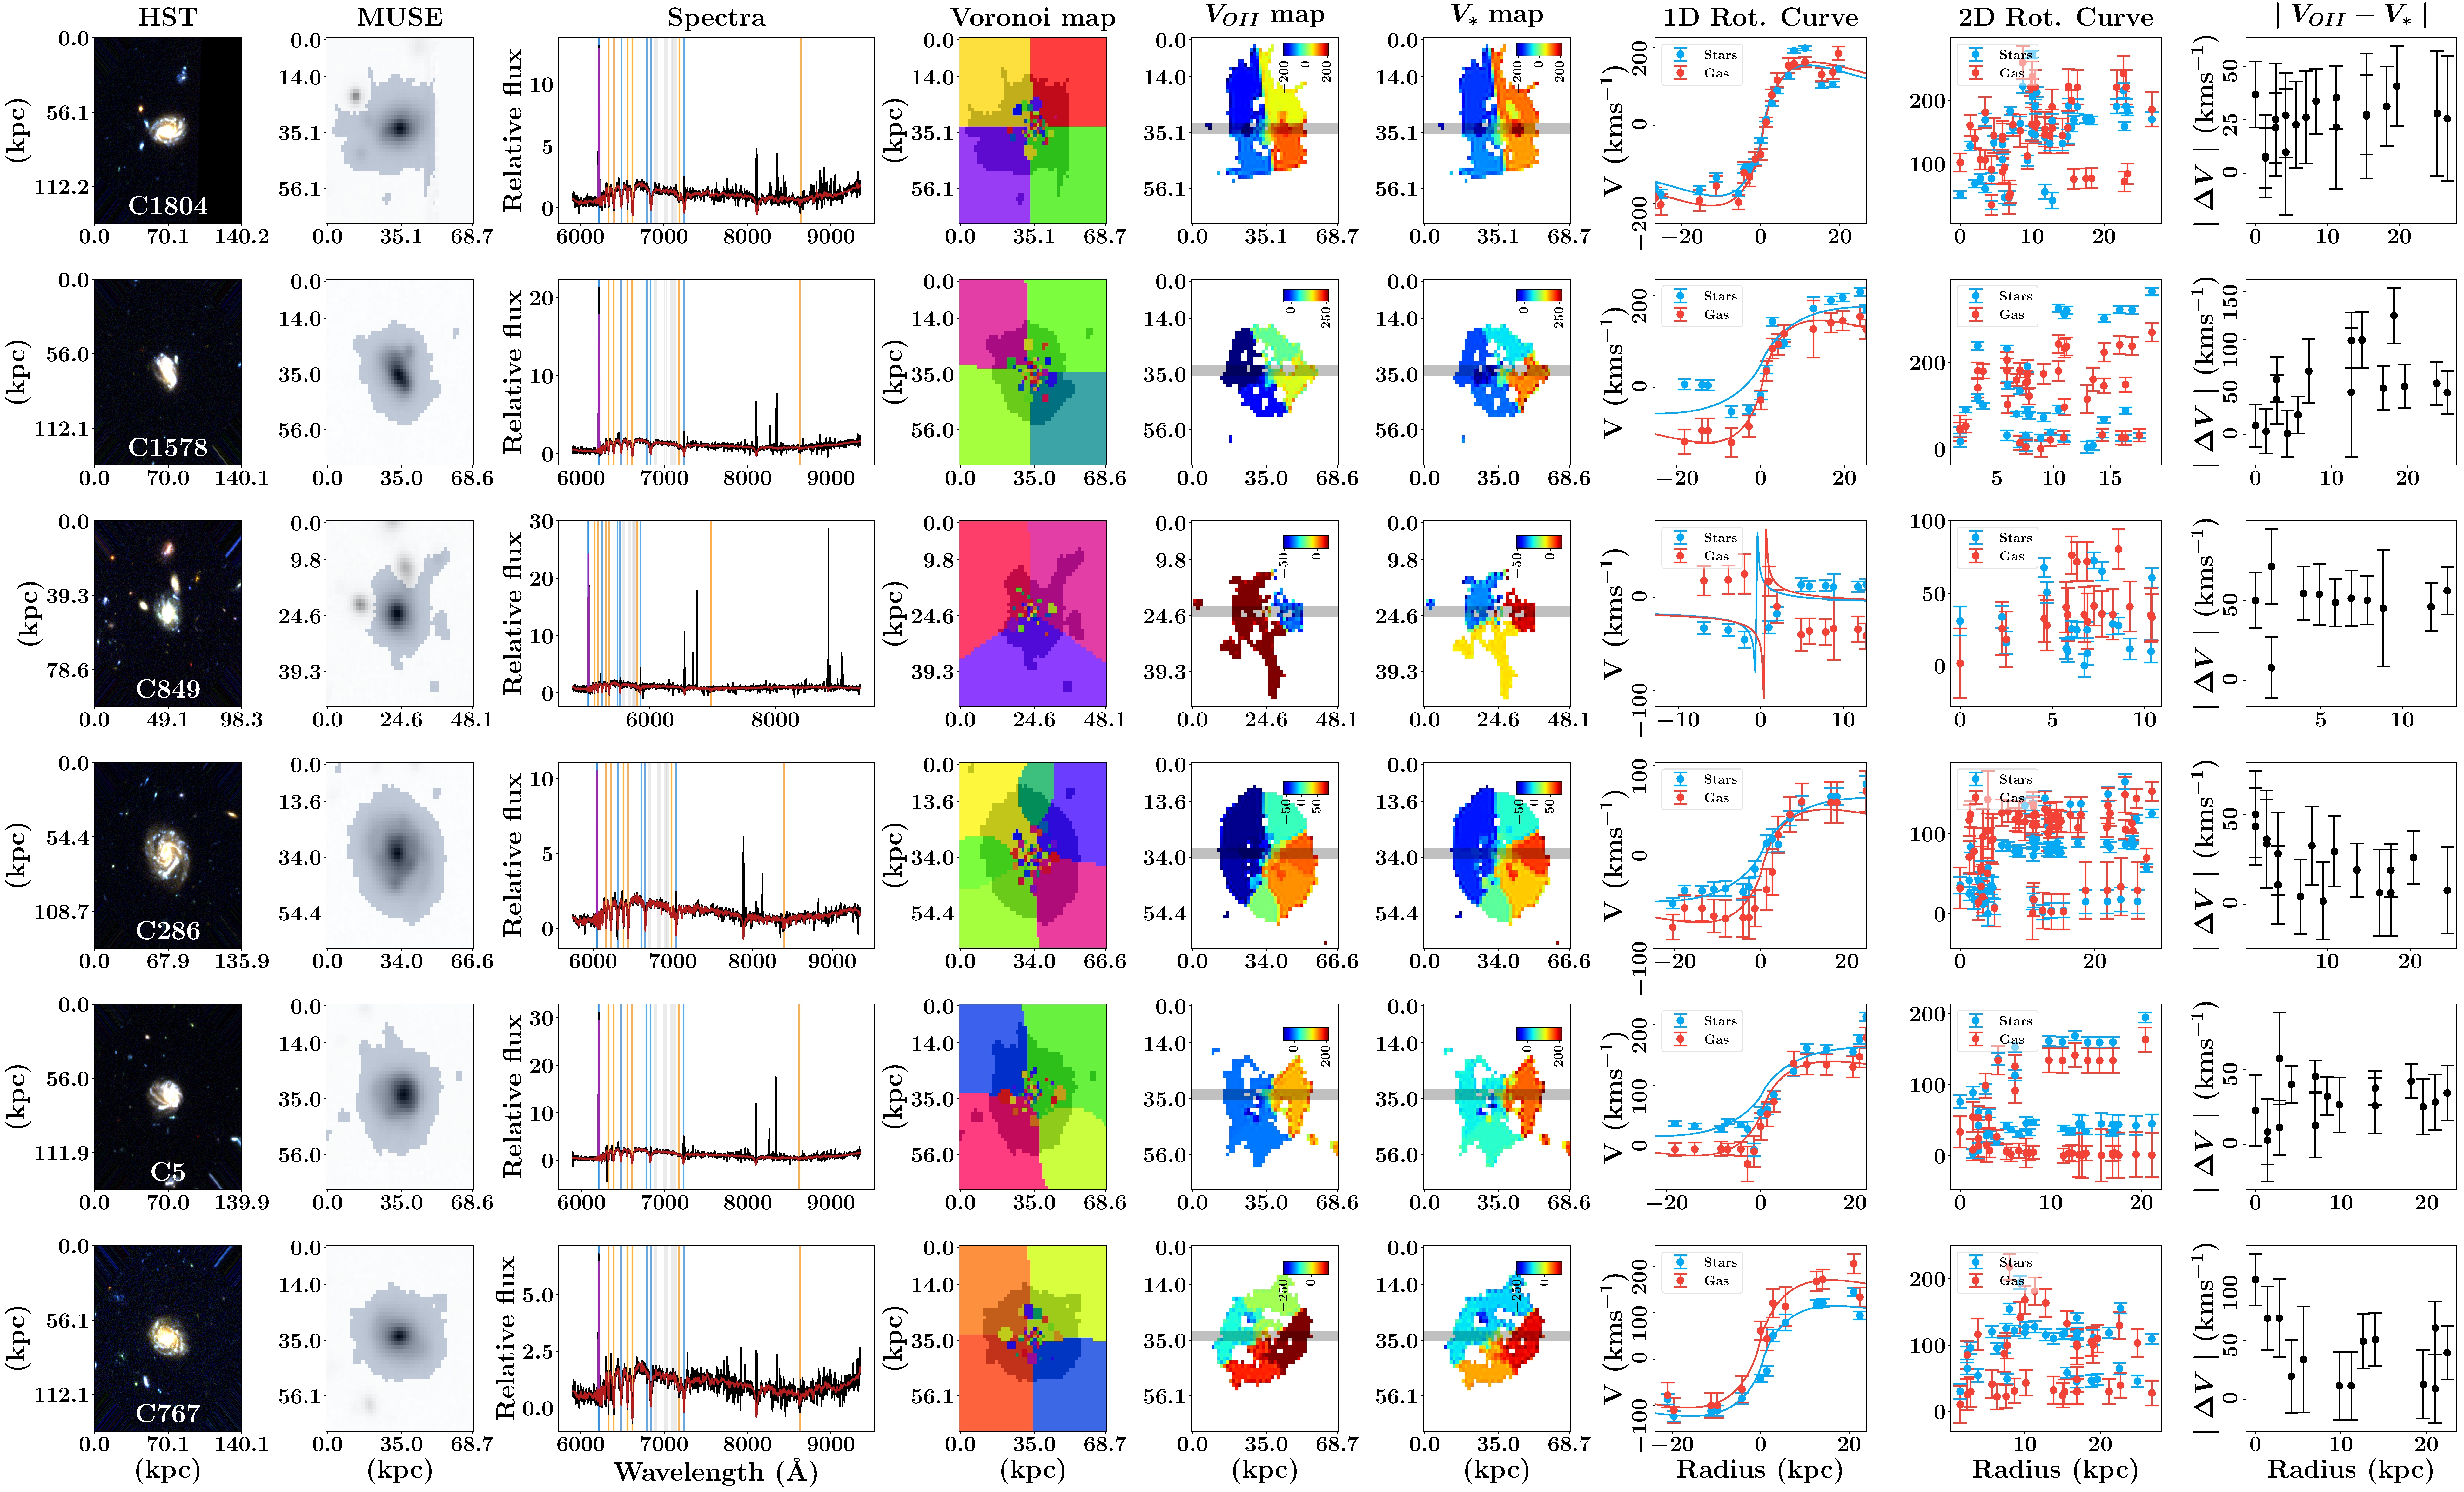
\includegraphics[width=1.0\textheight,height=0.6\textwidth]{data/spectra_complete_velocities}
%\vspace{-10ex}
\caption[Tully-Fisher]{Voronoi tessellation analysis for 6 galaxies. \textit{HST}: HST colour image and galaxy cube ID. \textit{MUSE}: collapsed optical image from MUSE spectroscopic data and segmentation map (grey). \textit{Spectra}: galaxy data (black); pPXF model (red); and emission (blue), absorption (orange), and iron (grey) spectral lines. \textit{Voronoi map}: Voronoi tessellated MUSE map and segmentation area. \textit{$V_{OII}$, $V_{*}$ maps}: velocity fields for galaxy. \textit{1D Rot. Curve}: rotation curve as defined by grey strips on velocity maps. \textit{2D Rot. Curve}: rotation curves from galaxy inclined-corrected map. \textit{$\mid V_{OII}-V_* \mid$}: stellar and gas velocity difference versus galaxy radius with data from 1D rotation curves.}
\label{fig:multiple_spectra}
\end{sidewaysfigure*}

\twocolumngrid

\subsubsection{Faber-Jackson}

\subsection{Applicability of locally derived scaling relations}

\subsection{Future studies}

Amongst the different types of cosmic structure within our universe, galaxies can be described as the most unique and diverse. With each containing countless numbers of stars and vast amounts of gas, dust, and dark matter \citep{carroll_astro}, it would be surprising if these various inner objects were not connected in any way.

Through observational astronomy the internal structure of galaxies and the motions of the internal objects can be studied and understood. With approximately ($2.0^{+0.7}_{-0.6}$) $\times 10^{12}$ galaxies in the universe up to redshift $z=8$ which in principle could be observed \citep{conselice_galaxynumber}, there is definitely not a lack of choice. What is important is how these objects are observed and how the collected data is later analysed. 

% There are a variety of methods 

% what are the variety of methods which can be used to study galaxies?

% Through observations of these galaxies, their structure and the motions of the objects within them can be studied to a great depth. As an example, if we took optical measurements of the stellar population, we could use that information to infer and estimate the potential age of the galaxy. We know that redder stars are older and bluer stars represent a younger set of objects \citep{carroll_astro}. Or if we wanted to know about the material composition or even the distance to a certain galaxy, we could split the collected light in a spectrograph to produce a spectrum. Values of redshift and the content of a galaxy can then be obtained by looking at the absorption and emission lines \citep{carroll_astro}.

The initial step one must take though is to understand the basics, therefore developing a comprehension of what a galaxy generally is and how they can be defined and placed into different categories. Once an appreciation is built for galactic classification, the intricacies of the inter-relationships can be explored further. 

%  for example how a galaxy evolves from the early stages of being a gas cloud to the eventual relation of the stellar population to that gas.

%%%%%%%%%% OLD REPORT %%%%%%%%%%

\subsection*{Galactic classification}

As stated previously, a galaxy can be quite broadly defined as a collection of gas, dust, stars and dark matter. But if a large enough sample was observed then one would begin to see that galaxies can be grouped and classified together.

The most general categorisation is called the \textit{Hubble Sequence} or the \textit{Hubble Tuning Fork} \citep{carroll_astro}. Developed by Edwin Hubble in 1926, galaxies can be roughly divided into ellipticals, spirals and irregulars (Fig. \ref{fig:hubble_tuning_fork}). With early Hubble type ellipticals along the horizontal handle, then the two prongs contain normal and barred spirals (later Hubble types), and irregulars form the third category. What can be seen from the Tuning Fork is a summarised view of the main galaxy types. However, in reality, there are more than the 11 groupings named.

The sequence itself does not show the evolution of the galaxies, rather it provides a way to view the different potential morphologies. So then, what does each grouping from the sequence actually represent? 

Starting with the most broad, irregulars are objects which do not fall into the two main galaxy types (ellipticals and spirals). Nevertheless, irregulars can in fact be split into two sub-categories depending on if a particular galaxy appears to have structure, such as spiral arms \citep{carroll_astro}. If there is structure then they would be Irr I galaxies, and if they appeared to be extremely disorganised then Irr II. Generally, irregulars are not particularly large, their diameters typically range from 1 to 10 kpc, and they have an absolute B-band magnitude of $-13$ to $-20$ mag.

% Some astronomers even argue that there is not a strong particular need for this grouping as these galaxies can fall into the spherical type \citep{carroll_astro}.

This classification by appearance can easily be extended to ellipticals and spirals, and their individual component composition can additionally be studied and explored. 

With ellipticals, they span from being virtually spherical (E0) to highly flattened (E7) collections of objects and material \citep{moore_databook}. Through observations of their stars, it can be seen that the majority of them are old, red types. This may be attributed to the amount of gas used in the initial stages of galactic stellar formation. If a larger proportion was used up initially then current observations would should the stellar-birthrate in ellipticals to be low \citep{carroll_astro}. This could additionally explain the lack of discs which can otherwise be seen in spiral galaxies, if there is not enough surrounding material then the disc and arms features would not be able to form.

Exploring spirals, they can be described as being composed of a central nucleus with a surrounding disc of material. This disc contains denser regions which forces matter to collapse and coalesce to form additional features. One particular spiral characteristic leads to a supplemental classification group, and that is whether the nucleus has a ``bar'' running through it. Observing and comparing the two different types, one finds that barred spirals appear to be more elongated along the bar axis than their non-barred counterparts. 

The other main attribute for spiral galaxies are the protruding arms surrounding the main bulge \citep{carroll_astro}. In the later type spirals (Sc and SBc) they have arms which are more loosely wound than the earlier types (Sa and SBa) \citep{moore_databook}.

It can be seen then that with more available ``raw'' gas and dust \citep{carroll_astro}, spirals in their various forms could be assumed to have an overall younger stellar population. It is within the arms of spiral galaxies that new stars are found to be created, however stellar birth is definitely not limited to just these regions. Inside the spiral structure the gravitational field allows for angular momentum to be transported outwards. Older and less massive stars in the galaxy produce a gravitational field which eventually leads to the shocking of interstellar gas \citep{binney_galaxies}. As a result the density of the gas in the arms increase and certain regions then collapse to form new, young, blue, and massive stars. 

There is therefore a range in the age of the stellar population in spiral galaxies. The spiral arms contain young stars whilst the central nucleus is akin to that of elliptical galaxies where they have an older population of stars and fewer new stars are born \citep{carroll_astro, binney_galaxies}.

These then are the general characteristics of galaxies, and whilst they can be classified based on their appearance, it is through studying their stellar populations that our understanding of them improves. 

% TODO if I am going to discuss galactic formation, should I have mentioned the earlier detail on how ellipticals form stars early on in the galaxies' history? 

\subsection*{Galactic stellar formation}

% this section shouldn't be called galactic stellar formation

One could argue that the main backbone in any galaxy lies with the gas and dust as without them there would be no stars and galaxies would simply not exist. There are many models which aim to provide an explanation for galactic evolution, from an initial proto-nebulae to structure. It would be difficult to detail them all, but beneficial to at least address some issues which would have to be answered by a comprehensive galactic evolution theory. 

One problem is deciding if an initial nebula collapses in free-fall or whether it goes through a slow and dissipative collapse \citep{carroll_astro}. If the time taken to cool the nebula significantly (cooling timescale) is much less than the time taken for free-fall, then the cloud would not be pressure supported and the collapse would be a rapid free-fall. On the other hand, if the cooling time exceeds the free-fall time then a rapid collapse cannot occur as the gas cannot radiate its energy away fast enough, therefore the gravitational potential energy released from a collapse will heat the nebula adiabatically. 

This is important to understand as from the heated and collapsed gas, the first stars can then be produced. It is not surprising then that a theory for galactic evolution should also be able to explain the rate of star formation. This rate can be described as a stellar birthrate function, $B(M,t)$, and be expressed as,
\begin{equation}
B(M,t)dM dt = \psi (t) \xi (M) dM dt, 
\label{eqn:stellar_birth_rate}
\end{equation}

where $\psi(t)$ is the star formation rate (SFR), $\xi (M)$ is the initial mass function (IMF), $M$ is the stellar mass, and $t$ is time \citep{carroll_astro}. 

Describing the physical meanings of the key terms: $B(M,t)$ is the number of stars per unit volume with masses between $M$ and $M+dM$ which are formed out of the interstellar medium (ISM) between time $t$ and $t+dt$, $\psi(t)$ is the rate per unit volume at which mass in the ISM is converted into stars, and $\xi(M)$ is the relative number of stars which form in each mass interval \citep{carroll_astro}. 

Additionally, assumptions can be made by researchers which subsequently leads to varying results \citep{carroll_astro}. Some astronomers say that the SFR is time-independent, whilst others describe it as exponentially decreasing with time, and a few even argue that it is proportional to a power of the surface mass density of the galactic disc. Then take the IMF, there is disagreement on the exact form it takes, some model it to be a power-law as a function of mass, but it is not clear if it also varies with time or location.

Through contentious debate and research, astronomers can continue to build these different models and theories which attempt to explain galactic evolution. Whilst on the other hand, the evolution of the stars themselves are known and better understood. 

In a brief overview: stars are born from an interstellar medium where the gas and dust coalesce, collapse and heat-up until a protostar is created. Depending on the initial mass of material used, the star can then take various paths which will affect its subsequent future \citep{mccoy_space_sciences}. To view the different stages of stellar evolution, Hayashi tracks and a Hertzsprung-Russell diagram can be paired together \citep{carroll_astro}. In doing so, one would find that the majority of stars lie on the main-sequence, including our own Sun.  

% If I need more discussion space, I could place the table in an appendix?

The classification of stars can be made with the \textit{Harvard Spectral Classification} where stars are classed by their spectral types (Table \ref{table:spectral_classification}). It essentially orders stars by their observed temperature and their internal composition. If a star's spectra was observed, it could be identified by the absorption and emission features found in the sequence.   

This therefore is one of ways to study the stellar population of a galaxy as the signatures of different spectral types can be matched up in a particular galaxy spectra. 

It is clear then that observational data would be required for own study of galaxies and the internal motions of the objects within them. 

\subsection*{Galactic data} 

For an investigation of galaxies, one would have to collect data optically and also spectroscopically. The former would be useful as it would allow for a quick identification of the galaxy based on its appearance, this could then be used to infer whether a galaxy would be worth studying. Spectroscopic data on the other hand would be important as a variety of information could be obtained such as the type of stars within a galaxy, the types of gas in the surrounding clouds, and also numerical values such as the redshift $z$. 

Astronomers on a daily basis employ an assortment of telescopes and spectrographs, but there are a few in particular which are worth discussing as they have produced remarkable datasets.

\subsubsection*{HUDF}

The Hubble Space Telescope (HST) has been operating since April 1990 and for the duration of that time it has collected over 50 terabytes of data \citep{mccoy_space_sciences}. From observing nebulae to attempts to detect extra-solar planets, HST has been used in a variety of searches. However, one of the most impressive and insightful uses of HST was the collection of the long-exposures taken in 1996 to produce the Hubble Deep Field (HDF). 

Through a combination of its visible and infrared cameras, the HDF was produced by piecing together different datasets which were collected over a period of 10 consecutive days \citep{mccoy_space_sciences, williams_hdp}. The four-band, 0.5 million s exposure revealed sources with redshifts $z>1$ which would have been difficult to view from ground-based observations \citep{beckwith_hudf}. 

% Expand on this section in the actual report i.e. the implications of HDF
% What regions of space was used to create the HDF? 

It is therefore unsurprising that another attempt was made in 2011 which resulted in the Hubble Ultra Deep Field (HUDF). This survey utilised 1 million s of exposure time on an 11 arcmin$^2$ area in the southern sky. Viewed again with four different filters, this survey resulted in at least 10,000 objects being detected in the field \citep{beckwith_hudf}. With a large majority being galaxies, the HUDF would be a prime dataset for a galactic study as there is such a large range of candidates which span the universe's history. 

% Should probably talk more about the HUDF and what the specs of it actually are, I'm just currently a bit conscious on the amount of space which I have left 

% why was the HUDF deep field commissioned?

\subsubsection*{MUSE}

In addition to optical observations, as noted previously, spectroscopic data should also be employed in a study of galaxies. One particular instrument which was used to acquire data on the HUDF region is the Multi-Unit Spectroscopic Explorer (MUSE) mounted to the Nasmyth platform on the Very Large Telescope (VLT) \citep{bacon_muse_proposal}. 

% provide some more history and specs for MUSE, reasons as to why it was commissioned 

The MUSE Hubble Ultra Deep Field Survey was performed over a two year timeframe from September 2014 to February 2017 \citep{bacon_muse_hudf}. It made use of 137 h of observation time and covers 90\% of the HUDF region. The 3D composite data cube mosaic made use of nine fields and represents the deepest spectroscopic survey ever performed. Both HST and MUSE HUDFs can be optically compared together, the latter is achieved by collapsing the cube axis containing the spectroscopic data into three components representing (R,G,B). Looking at both images (Figure \ref{fig:hst_muse_hdf}), the HST data appears to have more resolution whilst the MUSE objects are smeared out. However this is of no particular issue as the main use for MUSE is the manipulation of the spectra data which in turn will inform us on the optical data.

% TODO what is MUSE, problems, limitations of MUSE - why it is useful...etc

% what are the three dimensions of the 3D data MUSE cube? then what are the units of each dimension??

% in the full report, I might want to just put a table which provides all the main specifications for HST and MUSE

Through a coupling of both, the dynamics of stars and gas in galaxies can therefore be studied. The main analysis arising from the manipulation and comparison of different component areas of the spectra.


% Voigt profile fittings,

% Following this, Section \ref{sec:discussion} provides an exploration on the implications on the results obtained from the data analysis. Then the discussion will end on future work which can be performed to extend on the project.

\section*{Analysis} 
\label{sec:analysis}

The initial goal in the analysis was to reduce down the MUSE data cube into smaller cubes which contained individual galaxies. These could then be collapsed to produce a single galaxy integrated spectrum to represent the dynamics of the entire galaxy. Subsequently different fitting routines could be applied which would allow for a comparison of the gas to the stars in a galaxy.

\subsection*{Cube extraction}

To begin with, galaxies were identified from the 3D MUSE cube using \textit{SExtractor}; an automated routine which detects, de-blends, measures and classifies sources \citep{bertin_sextractor}. Employed in the astronomical software package \textit{GAIA} \citep{currie_starlink}, every potential galactic source was retrieved along with a ``segmentation map'' which discerns between multiple galaxies if several are close together. 

The final object list from SExtractor were compared and merged with a catalogue which contained every object identified in the HST HUDF frame. The latter would contain information such as initial guesses for redshifts, the magnitudes of the objects in the different wavelength filters, and various flux values for different emission and absorption lines.

% make sure the above caption actually makes sense

With every extracted galaxy, the signal-to-noise (S/N) could be calculated with the flux values from the catalogue. This was then plotted against the V-band magnitude (Figure \ref{fig:sn_vband}(a)), and one should find that as the S/N increases, the object should become brighter. A similar trend is also found if the S/N was measured using regions of the galaxy-integrated spectrum (Figure \ref{fig:sn_vband}(b)). The ``signal'' calculated by taking the median of the region and the ``noise'' as the standard deviation of a separate sky spectra. Both plots agree which implies that further analysis on the extracted galaxies should in theory produce sensible results. 

\subsection*{Line fittings and pPXF} 

After identifying the individual galactic objects from the MUSE cube, the spectroscopic data could then be extracted, manipulated and analysed by using different fitting routines: (i) [OII] doublet fittings, and (ii) \textit{pPXF} absorption and emission line fittings.

% and (iii) Voigt profile fittings.  

It would be quite non-sensical to use the entire catalogue of objects as there are more than 10,000 plus the majority are not high enough in S/N for spectra evaluation. Therefore several sample reducing methods were applied: (1) galaxies were sorted by redshift and then objects below $z<0.3$ ignored, (2) sample was then re-sorted by V-band magnitude and just the top 300 brightest objects extracted, and finally (3) the final set was found by considering galaxies with a magnitude brighter than 25.0 mag. 

With the reduced sample in hand, the model fitting analysis could then be performed.

% Give a table of the final galaxies considered in the Appendix?

% give reasonings for the sample reducing methods?

% the entire catalogue was sorted by the V-band magnitude and then reduced by choosing only the top 300

% Talk about what sample was used for the analysis, how it was chosen and the different parameters which were set and chosen 

\subsubsection*{Gaussian doublet fitting}

Through collapsing the entire galaxy into a single spectrum, one should find the [OII] doublet emission line to be the most prominent feature due to its large amplitude when compared to other spectral lines (Figure \ref{fig:ppxf_spectra}). This therefore allows it to be a useful tool for estimating the SFR, which in turn can be used as an indication of the evolutionary state of the galaxy \citep{maddox_oxygen}.

For every doublet fitting performed, the region $3600\times(1+z)$ {\AA} to $3750\times(1+z)$ {\AA} was extracted to isolate the peaks from other absorption or emission features. The peaks themselves have rest wavelengths 3727.092 {\AA} and 3729.875 {\AA} \citep{sdss_lines}. 

The following was applied as the model,
\begin{multline}
f_{\text{[OII]}}(x) = cx + \frac{I_1}{\sigma \sqrt{2\pi}} \exp{\Bigg(-\frac{(x-L_1)^2}{2\sigma^2}\Bigg)} \\
+ \frac{I_2}{\sigma \sqrt{2\pi}} \exp{\Bigg(-\frac{(x-L_2)^2}{2\sigma^2}\Bigg)},
\label{eqn:doublet}
\end{multline} 

where $x$ are the redshifted wavelengths, ${c}$ is a constant, ${I_1}$ and ${I_2}$ are scaling factors, $L_1$ and $L_2$ are the [OII] peaks multiplied by $(1+{z})$, and $\sigma$ is the quadrature sum of the fixed instrumental resolution $\sigma_{\text{inst}}$ and the deconvolved width of the doublet $\sigma_{\text{gal}}$ ($\sigma=\sqrt{{\sigma_{\text{gal}}}^2 + \sigma_{\text{inst}}^2}$).

% use NIST database as the reference when the US government shutdown is over

% provide constraints used in the doublet fitting?

After a successful fitting, the following variables would be outputted: $c$, $I_1$, $I_2$, $z$, and $\sigma_{\text{gal}}$. The latter two would become the most useful in later research. 

The redshifts along with the [OII] flux $f_{\text{[OII]}}(x)$ can be used to calculate the luminosity for the doublet, this luminosity can then be plotted against the redshifts (Figure \ref{fig:oiiluminosity_redshift}). What can be found is a general agreement that the galaxies follow the luminosity-redshift relation, thus the calculated parameters are sensible so they can be applied to other analysis routines.

\subsubsection*{pPXF fitting}

With the gas dynamics of galaxies represented through the width of the [OII] doublet, a comparison to galactic stars would require the width of the stellar spectra features. To obtain this, a Penalized Pixel-Fitting method (pPXF) can be applied, \cite{cappaellari_ppxf} describes the method and implementation in the form of a Python library \textit{pPXF}.

A reasonable initial test would be to pass an entire galaxy spectrum to the kinematics fitter and then examine the output to check if it seems reasonable. As well as a final model spectrum (Figure \ref{fig:ppxf_spectra}), pPXF also outputs its optimal variables and amongst them includes a velocity dispersion. However for these values and results to be comprehensible, one must be aware of what initial parameters are being passed to the fitting routine. 

An estimate of the redshift can be obtained from the previous [OII] doublet modelling, an instrumental resolution can be found by fitting a single Gaussian profile over the peak at $\sim6300$ {\AA} in a spectrum of the sky noise, and different template sets can be passed to the routine. 

% discuss the importance of a good template set

% place somewhere what the "widths" are the same as the standard deviations or "sigmas"

Whilst it may seem trivial to configure these values, the results obtained have not been logical. Using pPXF to estimate the gas population of a galaxy, an additional value can be obtained for the width of the [OII] doublet. This therefore allows us to plot both against each other where one should find a 1-to-1 positive linear trend. What is found instead is that both are not correlated (Figure \ref{fig:oii_widths}) which is a non-sensical result. 

In an attempt to remedy this issue, several options were explored. The first of which was to artificially create the [OII] feature with a known width and then apply pPXF, the output of this test resulted in yet again a meaningless result. It was then decided that the template spectra being used in the routine were not high enough spectral resolution, ideally one would use a set which has a greater value than the resolution of the MUSE data. 

% What is the MUSE instrumental resolution? 
% there are different spectral resolutions depending on what wavelength of data is being observed
% https://www.eso.org/sci/facilities/paranal/instruments/muse/inst.html

The initial template sets tested were the MILES stellar population models \citep{vazdekis_miles} and those by \cite{jacoby_spectra}, but these were found to be too low-resolution. The SYNTHE spectral library \citep{munari_synthe} has an incredibly high resolution of $R=20,000$, however it was difficult to integrate this into the pPXF routine. What was decided on was the Indo-US Library of Coud{\'e} Feed Stellar Spectra \citep{valdes_coude} library with $R\sim4200$, this should be high enough to not produce additional problems.

\begin{figure}
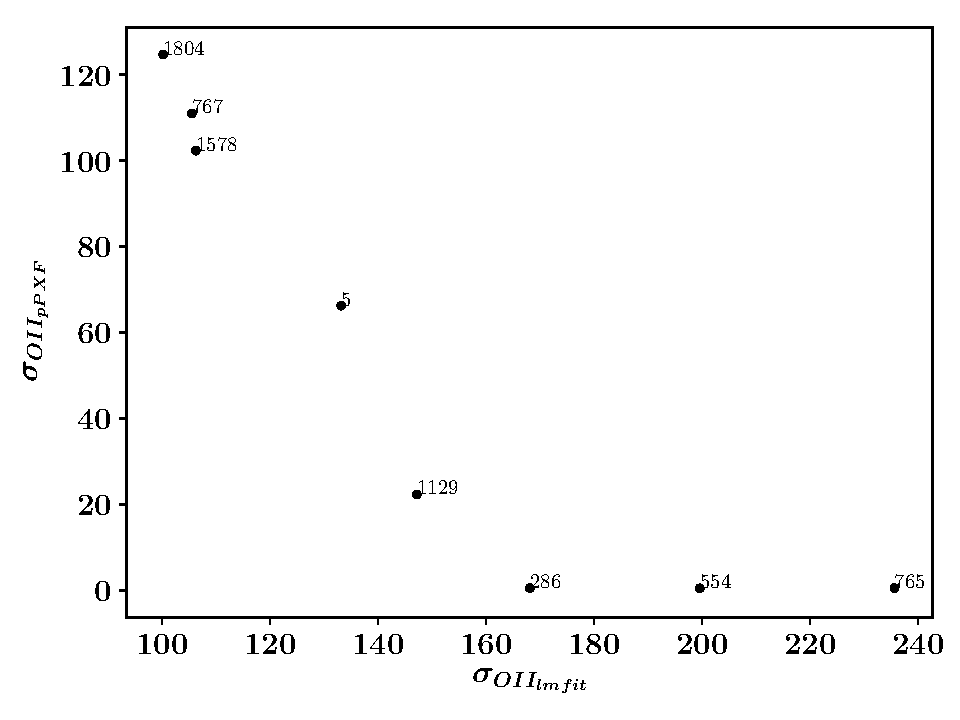
\includegraphics[width=1.0\linewidth]{data/oii_ppxf_vs_oii_lmfit}
\caption{The widths of the [OII] doublets obtained from the Gaussian modelling (labelled \textit{lmfit}) plotted against the widths found from the gas population fitter in pPXF. A linear trend is expected, however a failure in the set-up of pPXF has produced the illogical results as shown in the plot.}
\label{fig:oii_widths}
\end{figure}

The Coud{\'e} library has yet to be fully tested as other limitations of pPXF were explored. One question which arose was what are the computational limits of pPXF? Amongst the variables outputted, there are associated uncertainties on those values. How could they be trusted? 

Another synthetic test of pPXF was performed where 10 galaxy spectra were each perturbed 300 times. Random Gaussian noise was added sequentially until the spectra were unrecognisable. During each perturbation the spectra was passed to pPXF and all associated outputs were saved and recorded. This allowed for the S/N to be plotted against the modulus difference between the original optimal line width and the values from the perturbation (Figure \ref{fig:sn_difference}). One finds that as the S/N decreases, the difference (or fractional error) increases dramatically. This is attributed to the fact that there would not be enough resolution for emission or absorption features to be discerned. It can be seen then that one must use data with a high enough S/N for pPXF to be above this high error zone.

% Provide values for the instrumental and template resolutions?

Whilst it can be understood what type of data should be passed to the pPXF routine, the routine itself still needs more unravelling if accurate and precise results are wanted in the comparisons of gas and stellar dynamics in galaxies.

%\subsubsection{Voigt fitting}

%\section{Discussion} 
%\label{sec:discussion}
%
%This is where the discussion section would be

\section{Conclusions}
\noindent
In conclusion, the dynamics of gas and stars within galaxies can be explored by analysing their spectra. Through reducing down the MUSE HUDF galaxy sample from $\sim10,000+$ to a small handful, the individual galaxies can have their [OII] peak fitted for, and then the spectra can be passed onto a stellar-dynamics fitting routine, pPXF. The key issues encountered in this stage of the project were based around the proper-running of pPXF, various tests were performed and a higher resolution template set was chosen, however the problems still remain and more work will be required to solve them.

\begin{acknowledgments}
The author would like to thank Dr.~M.~Swinbank and Alfie Tiley for their continual help and support throughout the project period.
\end{acknowledgments}

\bibliographystyle{agsm}
\bibliography{stars_gas_dynamics}

\clearpage

\appendix

\onecolumngrid
\section*{Appendices}
\section{Remaining galaxies} \label{appendix:rest_of_final_sample}
\noindent
The remaining 9 objects from the final reduced sample of 35 galaxies are presented in Table \ref{table:rest_of_final_sample}. These 9 are part of 20 which could not be analysed due to lack of signal-to-noise or lack of a prominent [OII] emission feature.

\begin{table*}[h!]
\centering
\begin{tabular}{c@{\hskip 10pt}c@{\hskip 10pt}c@{\hskip 10pt}c@{\hskip 10pt}c@{\hskip 10pt}c@{\hskip 10pt}c@{\hskip 10pt}c@{\hskip 10pt}c@{\hskip 10pt}c} 
 \hline
 \textbf{Cube ID} & \textbf{RAF ID} & \textbf{RA (deg)} & \textbf{Dec. (deg)} & \textbf{F606W mag.} & \textbf{$\boldsymbol{z}$}  \\ [0.5ex] 
C1411 & 20647 & 53.16431016 & -27.81082586 & $24.465(4)$ & $0.73503(6)$ \\ 

C943 & 6028 & 53.16620903 & -27.7939202 & $24.427(7)$ & $1.036159(9)$ \\ 

C1559 & 20306 & 53.16418209 & -27.81846837 & $25.402(7)$ & $1.09406556(0)$ \\ 

C543 & 22939 & 53.18402132 & -27.79150708 & $24.956(5)$ & $1.22018(3)$ \\ 

C1423 & 20544 & 53.16311572 & -27.81360388 & $24.459(3)$ & $1.42504(2)$ \\ 

C606 & 9791 & 53.1648948 & -27.77873099 & $25.17(1)$ & $0.98091(1)$ \\ 

C627 & 8908 & 53.15398319 & -27.77098973 & $24.666(8)$ & $0.83200(4)$ \\ 

C400 & 8559 & 53.15986702 & -27.76684123 & $24.615(7)$ & $1.03670(3)$ \\ 

C1134 & 2795 & 53.16638743 & -27.80182796 & $25.17(1)$ & $0.6820(1)$ \\ 

C1225 & 1742 & 53.16803964 & -27.80741481 & $24.014(4)$ & $0.30996(3)$ \\ 
 \hline
\end{tabular}
\caption{Remaining 9 objects from the 20 non-analysed galaxies which were not shown in Table \ref{table:final_sample}. Columns show the working cube ID, the ID from the UVUDF Catalogs \citep{2015AJ....150...31R} (RAF ID), the object right ascension (RA) and declination (Dec.), the magnitude of the object in the HST F606W filter, and the calculated galaxy redshift ($z$). Total sample contained 35 objects, 15 of which had high enough signal-to-noise in their spectra for the gas and stellar components to be analysed.}
\label{table:rest_of_final_sample}
\end{table*}

\end{document}